%%%%%%%%%%%%%%%%%%%%%%%%%%%%%%%%%%%%%%%%%
% Short Sectioned Assignment LaTeX Template Version 1.0 (5/5/12)
% This template has been downloaded from: http://www.LaTeXTemplates.com
% Original author:  Frits Wenneker (http://www.howtotex.com)
% License: CC BY-NC-SA 3.0 (http://creativecommons.org/licenses/by-nc-sa/3.0/)
%%%%%%%%%%%%%%%%%%%%%%%%%%%%%%%%%%%%%%%%%

\documentclass[paper=a4, fontsize=11pt]{book} % A4 paper and 11pt font size
\usepackage[T1]{fontenc} % Use 8-bit encoding that has 256 glyphs
\usepackage[utf8]{inputenc}
\usepackage{fourier} % Use the Adobe Utopia font for the document - comment this line to return to the LaTeX default
\usepackage{listings} % para insertar código con formato similar al editor
\usepackage[spanish, es-tabla]{babel} % Selecciona el español para palabras introducidas automáticamente, p.ej. "septiembre" en la fecha y especifica que se use la palabra Tabla en vez de Cuadro
\usepackage{url} % ,href} %para incluir URLs e hipervínculos dentro del texto (aunque hay que instalar href)
\usepackage{graphics,graphicx, float} %para incluir imágenes y colocarlas
\usepackage[gen]{eurosym} %para incluir el símbolo del euro
\usepackage{cite} %para incluir citas del archivo <nombre>.bib
\usepackage{enumerate}
\usepackage{csquotes}
\usepackage{hyperref}
\hypersetup{
	colorlinks,	% false: boxed links; true: colored links
	breaklinks,
	citecolor=black,
	linkcolor=black,	% color of internal links
	urlcolor=black		% color of external links
}
\renewcommand{\familydefault}{\sfdefault}
\usepackage{fancyhdr} % Custom headers and footers
\pagestyle{fancy}
\fancyhf{}
\fancyhead[LO]{\leftmark}
\fancyhead[RE]{\rightmark}
\fancyhead[RO,LE]{\textbf{\thepage}}
\renewcommand{\headrulewidth}{0pt} % Remove header underlines
\renewcommand{\footrulewidth}{0pt} % Remove footer underlines
\setlength{\headheight}{13.6pt} % Customize the height of the header

\begin{document}

	% Plantilla portada UGR
	\begin{titlepage}
	
	\newlength{\centeroffset}
	\setlength{\centeroffset}{-0.5\oddsidemargin}
	\addtolength{\centeroffset}{0.5\evensidemargin}
	\thispagestyle{empty}
	\noindent\hspace*{\centeroffset}
	
	\begin{minipage}{\textwidth}	
		\centering
		
\includegraphics[width=0.8\textwidth]{imagenes/logo_ugr.jpg}\\[1.4cm]
		\textsc{\Large TRABAJO DE FIN DE GRADO\\[0.2cm]}
		\textsc{INGENIERÍA EN INFORMÁTICA}\\[1cm]
		{\Huge\bfseries Meta-Dynasystem\\}
		\noindent\rule[-1ex]{\textwidth}{3pt}\\[3.5ex]
		{\large\bfseries Distro \textit{GNU/Linux} propia con actualizaciones \textit{Over-the-air}}
	\end{minipage}
	
	\vspace{2.5cm}
	\noindent\hspace*{\centeroffset}\begin{minipage}{\textwidth}
	\centering
	
	\textbf{Autor}: {Adrián Morente Gabaldón}\\[2.5ex]
	\textbf{Director}: {Juan Julián Merelo Guervós}\\[1.5cm]
	
\includegraphics[width=0.3\textwidth]{imagenes/etsiit_logo.png}\\[0.1cm]
	\textsc{Escuela Técnica Superior de Ingenierías Informática y de Telecomunicación}\\
	\textsc{---}\\
	Granada, junio de 2018
	\end{minipage}

\end{titlepage}
	
	% Plantilla prefacio UGR
	\chapter*{}

\cleardoublepage
\thispagestyle{empty}

\begin{center}
	{\large\bfseries Meta-Dynasystem}\\
\end{center}
\begin{center}
	Adrián Morente Gabaldón\\
\end{center}

%\vspace{0.7cm}
\noindent{\textbf{Palabras clave}: GNU/Linux, distribución Linux, dispositivo embebido, actualizaciones OTA, Yocto Project, Mender.io, Dynasystem}\\

\vspace{0.7cm}
\noindent{\textbf{Resumen}}\\

Actualmente la sociedad se encuentra cada vez más sumida en un ecosistema total de computación ubicua, rodeándose de pequeños computadores con funciones muy específicas y determinadas, cuyas interacciones con el entorno hacen que su naturaleza tecnológica pase desapercibida para los humanos. Se tratan de los llamados \textbf{sistemas embebidos}, que plantean nuevos retos al gremio de ingenieros de cualquier tipo, quienes intentan maximizar la productividad e innovar en funcionalidad además de ahorrar consumo y precios de coste.\\

El proyecto \textit{\textbf{Meta-DYNAsystem}} nace como solución propuesta a la implementación de una \textbf{infraestructura virtual} para un sistema dedicado de este tipo.\\

Persigue el desarrollo de una nueva distribución propia basada en GNU/Linux que dote al dispositivo físico de ligereza, eficacia y el rendimiento necesario para embeber una aplicación de \textbf{tiempo real}. Además, presta especial atención a detalles estéticos que hacen más natural esta interacción con el sistema y presenta la información de forma más atractiva para el usuario.\\

Finalmente, intenta innovar en el uso de distribuciones embebidas dotándose de \textbf{actualizaciones \textit{Over-the-Air}} centralizadas a través de un servidor dedicado.\\

\cleardoublepage
\thispagestyle{empty}

\begin{center}
	{\large\bfseries Meta-DYNAsystem}\\
\end{center}
\begin{center}
	Adrián Morente Gabaldón\\
\end{center}

%\vspace{0.7cm}
\noindent{\textbf{Keywords}: GNU/Linux, Linux distro, embedded device, OTA updates, Yocto Project, Mender.io, Dynasystem}\\

\vspace{0.7cm}
\noindent{\textbf{Abstract}}\\

Nowadays, society is increasingly immersed in an ubiquitous computing ecosystem, surrounding itself with small computers with very specific and determined functions, whose interactions with the whole environment make their technological origin goes unnoticed by humans. These devices are known as \textbf{embedded systems}, which pose new challenges to the engineers' guild of any kind, who try to maximize productivity and innovate in functionality, in addition to saving consumption and cost prices.\\

The \textbf{\textit{Meta-DYNAsystem}} project was born as a proposed solution to the implementation of a \textbf{virtual infrastructure} for a dedicated system of this kind.\\

It pursues the development of a new proprietary GNU/Linux-based distribution that endows the physical device with lightness, effectiveness and the necessary performance to embed a real-time application. Moreover, it attends to aesthetical details which make this interaction with the system more natural and it shows the information in a more attractive way to the user.\\

Finally, it tries to innovate in the use of embedded distributions, equipping itself with \textbf{\textit{Over-the-Air} updates} centralized through a dedicated server.

\chapter*{}
\thispagestyle{empty}

\noindent\rule[-1ex]{\textwidth}{2pt}\\[4.5ex]

Yo, \textbf{Adrián Morente Gabaldón}, alumno de la titulación Grado en Ingeniería Informática de la \textbf{Escuela Técnica Superior
de Ingenierías Informática y de Telecomunicación de la Universidad de Granada}, con DNI 77139229N, autorizo la
ubicación de la siguiente copia de mi Trabajo Fin de Grado en la biblioteca del centro para que pueda ser
consultada por las personas que lo deseen.

\vspace{6cm}

\noindent Fdo: Adrián Morente Gabaldón

\vspace{2cm}

\begin{flushright}
Granada a 18 de junio de 2018.
\end{flushright}


\chapter*{}
\thispagestyle{empty}

\noindent\rule[-1ex]{\textwidth}{2pt}\\[4.5ex]

D. \textbf{Juan Julián Merelo Guervós}, Profesor del Área de Ingeniería Informática del Departamento de Arquitectura y Tecnología de Computadores de la Universidad de Granada.

\vspace{0.5cm}

\textbf{Informa:}

\vspace{0.5cm}

Que el presente trabajo, titulado \textit{\textbf{Meta-Dynasystem}}, ha sido realizado bajo su supervisión por \textbf{Adrián Morente Gabaldón}, y autorizo la defensa de dicho trabajo ante el tribunal que corresponda.

\vspace{0.5cm}

Y para que conste, expide y firma el presente informe en Granada a 18 de junio de 2018.

\vspace{1cm}

\textbf{El director:}

\vspace{5cm}

\noindent \textbf{Juan Julián Merelo Guervós}

	\newpage
	
	% Índice de contenidos
	\tableofcontents
	\newpage

	% Índice de imágenes y tablas
	\listoffigures
	\newpage
	
	% Introducción: resumen e implementación para la empresa
	\chapter{Introducción}

Este Trabajo de Fin de Grado ha sido realizado íntegramente por mi persona, Adrián Morente Gabaldón, en colaboración con la empresa \textit{Synergy Movement Technologies 3000 S.L.} durante el período laboral mantenido con dicha compañía. El proyecto nace como solución propuesta a una parte del desarrollo de DYNAsystem \cite{dynasystem-web}, un dinamómetro funcional en forma de estación orientado al rendimiento deportivo y al tratamiento fisioterapéutico, el cual concentra la mayoría de los modos de entrenamiento que pueden encontrarse en un gimnasio, embebidos en forma de \textit{``caja negra''} y con un factor de forma y tamaño fácilmente integrables en cualquier entorno. Además, dada la naturaleza electrónica de estos dispositivos, tienen la capacidad de mostrar en tiempo real los datos que están siendo producidos por el usuario (como las fuerzas y velocidades medias y máximas, trabajo, número de repeticiones, tiempo de entrenamiento, etc.). Por otro lado, el control de dicho dispositivo se realiza a través de una aplicación embebida con interacción táctil, desde la que se configuran todos los ejercicios y rutinas deseadas por el usuario.\\

Dicha empresa llegó a vender a nivel internacional; pero atravesó diferentes fases temporales, cambiando de administración y nombre en un par de ocasiones, al igual que el producto (que también pasó por diferentes implementaciones), lo que derivó en la decisión de paralizar la venta de estos dispositivos. De esta forma sería factible realizar una re-formulación al completo de sus máquinas, mejorando tanto en \textit{potencia}, \textit{funcionalidad} y \textit{estética} como en \textit{reducción de costes y consumo}.\\

Una de las medidas que podrían ayudar a este rediseño sería la implantación de una infraestructura virtual diferente: un sistema operativo adaptado por y para la compañía, moderno y libremente personalizable. De esta forma, además de ejecutar la aplicación embebida que necesita el sistema para ser utilizado, el dispositivo podría constar de valores añadidos como animaciones de carga o \textbf{actualizaciones remotas} para solventar problemas de software y añadir nuevas funcionalidades a lo largo del tiempo.\\

En este documento hablaremos de los requisitos que se plantearon inicialmente para dicha infraestructura del producto (obviando otros aspectos del producto como el diseño estructural o la implementación de la propia aplicación embebida), trataremos el análisis que realicé y discutiremos las decisiones tomadas por mi parte para solucionar los problemas a lo largo del desarrollo. Finalmente, estimaremos un presupuesto del proyecto para éste y cualquier otro propósito general.\\

Cabe destacar que el proyecto es libre \textit{(bajo la licencia LGPL v3.0)} y está alojado en mi perfil de \textit{Github} \cite{github-adrian} con el consentimiento de la empresa, lo cual hay que agradecer por todas las ventajas que ello comporta.

\newpage
	
	% Estado del arte: situación actual de la tecnología, problemas que se desean resolver con el proyecto. Dispositivos embebidos. Definición, características y necesidades.
	\chapter{Estado del arte}

Dada la naturaleza del producto, a lo largo del proyecto hablaremos largo y tendido sobre \textbf{dispositivos embebidos}, y por qué no, del \textbf{\textit{Internet de las Cosas}}, dado que pese a ser una máquina orientada al tratamiento del ejercicio físico requiere de conectividad, procesamiento de datos y transmisiones de información. Con el creciente ritmo al que progresa el ya famoso concepto \textit{``Internet de las Cosas''} (en inglés, \textit{IoT, Internet of Things}), se está apreciando un grandioso crecimiento en el desarrollo de los dispositivos y sistemas embebidos y/o de tiempo real.\\

De hecho, como dice \textit{Bruce Powel Douglass} hoy en día encontramos sistemas de este tipo que varían en tamaño y rendimiento, desde un reloj de muñeca inteligente hasta la automatización de los sistemas de control de una central nuclear \cite{real-time-uml-introduction}.\\

Por otro lado, según \textit{Matthew Evans}, el paradigma del \textit{IoT} nos permite ser más eficientes en tiempo y recursos a la hora de hacer las cosas \cite{whats-iot}. Se debe a que es más rápido implementar un sistema dedicado con unas necesidades muy claras a analizar y constituir un sistema completo de otro tipo. Esto deriva directamente en ahorro de producción y por tanto en unos márgenes de beneficio más flexibles para la empresa.\\

\section{Situación actual de la tecnología}

Como también dice \textit{Douglass}, hoy en día podemos encontrar sistemas dedicados y aplicaciones de tiempo real para todo propósito y en cualquier factor de forma. Por ejemplo, veamos algunos casos llamativos de hoy en día:\\

Un ejemplo de sistema empotrado podría ser el que encontramos en algunos negocios de comida rápida (en este caso, \textbf{\textit{McDonald's}}), que disponen de pantallas táctiles de gran tamaño permitiendo al usuario realizar su pedido a través de éstas, y posteriormente pasar por caja a recogerlo. Como sistema dedicado, se trata de un tipo de dispositivos con una utilidad muy específica y aislada, por lo que su implementación debe centrarse siempre en la máxima representación de ésta.

\begin{figure}[H]
	\centering
	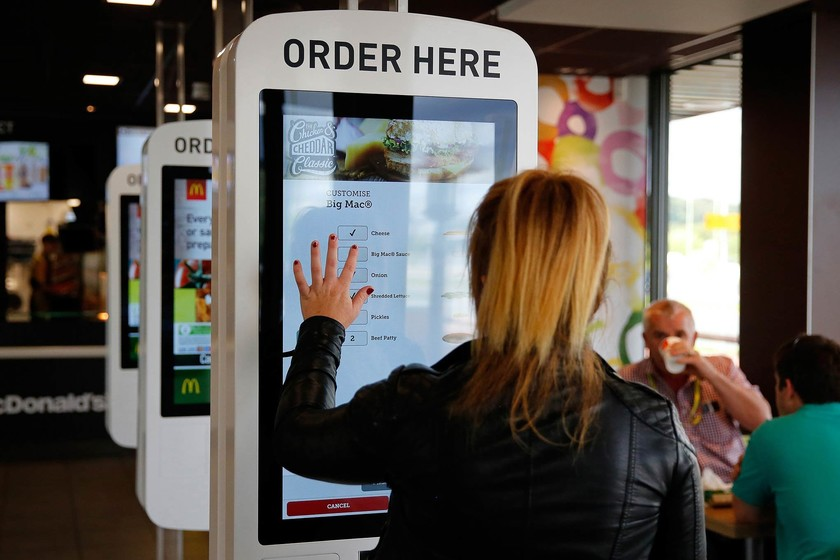
\includegraphics[width=0.75\linewidth]{imagenes/pedido-pantalla-tactil.jpg}
	\caption{Pantallas táctiles para realizar pedidos en McDonald's - Fuente: \textit{Mientras Tanto En México} \cite{mcdonalds-pantalla-tactil-pedidos}}
\end{figure}

Por otra parte, nos encontramos con la empresa alemana \textbf{\textit{gridX}} \cite{gridx}. Se trata de una empresa proveedora de energía limpia en Alemania que, además de apostar por las energías renovables y su administración de forma transparente, comercializan el dispositivo \textbf{gridBox}. Se trata de un sistema embebido que actúa a modo de contador y administrador inteligente con todo el consumo de dicha energía, optimizando el uso de ésta en el hogar.

\begin{figure}[H]
	\centering
	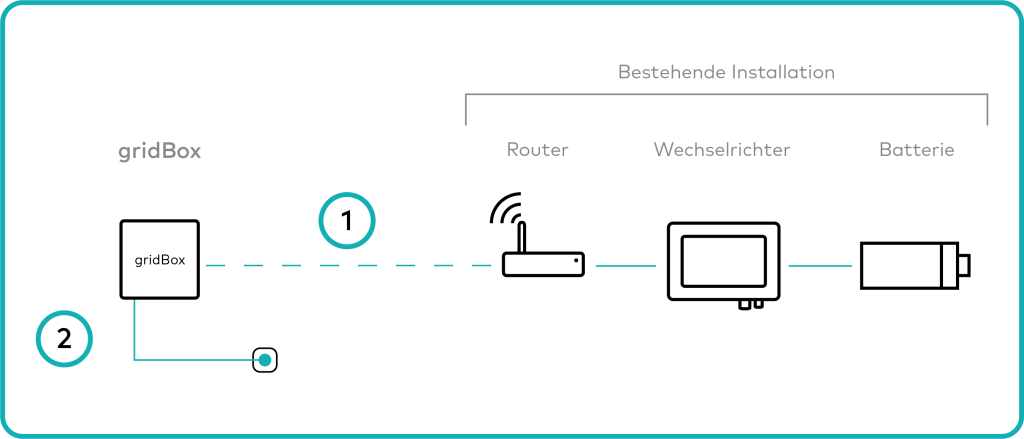
\includegraphics[width=0.75\linewidth]{imagenes/gridbox-utility.png}
	\caption{Instalación de gridBox en el hogar. De una toma de corriente a todos los dispositivos, pasando por el router - Fuente: \textit{Web oficial de gridX} \cite{gridbox}}
	\label{gridbox-installation}
\end{figure}

Además de ser un sistema dedicado con este propósito tan específico, implementa conexión de red para poder monitorizar los datos y transferirlos a aplicaciones de móvil y/o escritorio a los dueños de la casa. Y por último, el producto lleva integrado un sistema de actualizaciones \textit{OTA} con \textit{Mender.io}, herramienta de la que hablaremos extensamente más adelante.\\

A modo de último ejemplo, nos encontramos con \textbf{\textit{Kinestral}} \cite{kinestral}; una compañía con sedes en Norteamérica y Taiwan que focaliza su negocio en \textit{la transformación del cristal}. Comercializan el producto \textbf{\textit{Halio}}, que se trata de una especie de vidrio inteligente para cualquier propósito (sobre todo, el de la instalación en edificios) que posee la particularidad de \textbf{oscurecerse automática o manualmente} para sombrear y reducir el impacto de los deslumbramientos de la luz solar.

\begin{figure}[H]
	\centering
	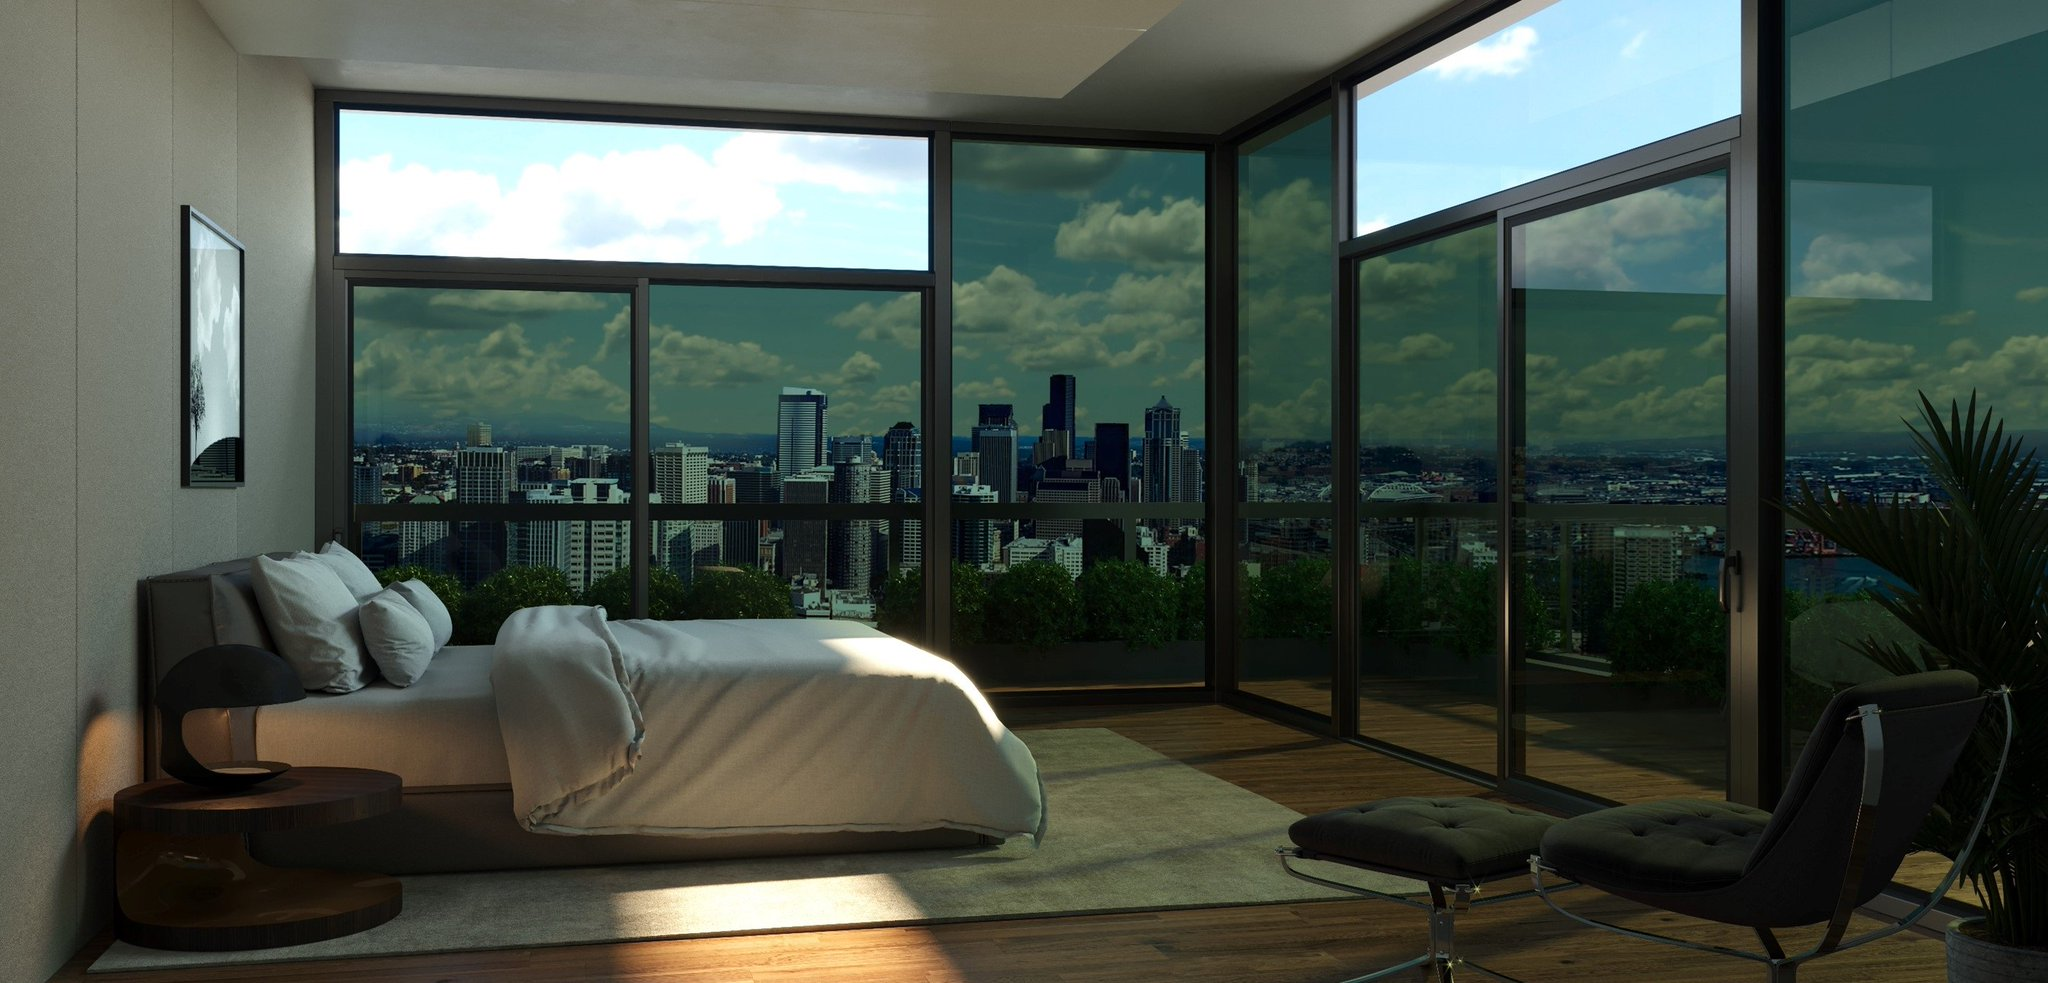
\includegraphics[width=0.8\linewidth]{imagenes/halio-glass.jpeg}
	\caption{Ejemplo de instalación de Halio Glass en el hogar - Fuente: \textit{Cuenta de Twitter oficial de Halio Glass (producto de Kinestral)} \cite{halio-glass}}
	\label{halio-glass}
\end{figure}

Además de esta funcionalidad tan curiosa e innovadora, incorporan la conexión con una aplicación móvil desde la que poder controlar de manera independiente cada uno de los paneles instalados en el edificio. Por último, también incorporan un sistema de actualización basado en \textit{Mender.io}.\\

\noindent\makebox[\linewidth]{\rule{\textwidth}{0.4pt}}\\

Una vez vistas algunas implementaciones de la tecnología, dado el propósito del proyecto en este apartado tenemos que distinguir entre dos grandes campos, \textbf{sistemas operativos embebidos} y \textbf{métodos de actualización}.\\

Antes de hablar de sistemas operativos empotrados, debemos concretar la idea de ``dispositivo embebido'' (o \textit{dedicado}) como tal. Para \textit{Jean Paul Calvez}, consiste en lo siguiente:

\begin{quotation}
	``Un sistema dedicado quiere decir que éste es desarrollado para satisfacer una necesidad muy concreta en un momento dado. Su límite de operatividad está definido en varios años o décadas, por lo que la durabilidad es importante. El sistema debería ser \textit{lo más perfecto posible}, siendo lanzado en su versión final con tecnologías actuales. Sus posibilidades de futuro desarrollo están limitadas a unas pocas mejoras para la misma aplicación. Por lo tanto, ni se trata de un ordenador de propósito general ni de un prototipo que funciona bien solo en un momento concreto. [...] La técnica implementada ha de ser correcta y adecuada para reducir costes y tiempo de desarrollo.'' - \textit{Jean Paul Calvez} \cite{embedded-real-time-systems-embedded-systems}
\end{quotation}

Entre las técnicas de implementación se encuentran el uso de sistemas completos (como microcomputadores, terminales o sistemas de procesamiento de imágenes) en contraposición al uso conjunto de placas de desarrollo, fuentes de alimentación y placas con microprocesador entre otras herramientas.\\

En cuanto a hardware suele darse el caso de \textbf{la reutilización}, no ya en el software; dado que en el primer caso es mucho mayor el coste de la creación de nuevos componentes, por lo que se prefiere reutilizar cosas que ya existen.\\

\noindent\makebox[\linewidth]{\rule{\textwidth}{0.4pt}}\\

Por una parte, los dispositivos embebidos están teniendo un gran crecimiento dadas las mejoras computacionales de rendimiento y consumo, permitiendo desarrollar sistemas aislados que desempeñan funciones muy específicas, como recopilar datos y transmitirlos (como una granja de dispositivos que implementan el protocolo \textit{ZigBee} \cite{zigbee-products}), o actuar de entorno multimedia para diversos fines (como los sistemas de navegación automovilísticos inteligentes, a menudo programados utilizando \textit{Qt Automotive Suite} \cite{qt-automotive}).\\

Principalmente, estos productos se desarrollan a partir de un \textbf{ordenador de placa reducida} (en inglés: \textit{Single Board Computer}, o \textit{SBC}); como lo son la \textit{Raspberry Pi} \cite{raspberry-pi}, la \textit{Tinker Board} de \textit{ASUS} \cite{asus-tinkerboard} o \textit{Arduino} en sus diferentes versiones \cite{arduino-store}. O bien, el equipo encargado de desarrollar el producto puede optar por diseñar una placa a medida que satisfaga las necesidades del proyecto. Para ésto, es necesaria una gran estimación de las ventajas con respecto al precio, y un desarrollo de software muy estrechamente ligado al del hardware.\\

Ahora bien, sobre estas plataformas hardware se pueden utilizar diferentes sistemas operativos, dando prioridad a la elaboración de uno propio a partir de diversas herramientas (como \textit{OpenEmbedded/Yocto Project} \cite{yocto-project}, \textit{Buildroot} \cite{buildroot} o \textit{Linux from scratch} \cite{linux-from-scratch}); ya que aseguran una mayor modularidad y ligereza en cuanto a dependencias (no se instala nada que no sea necesario). Estas tecnologías suelen ser de código abierto, libres y gratuitas, aunque existen alternativas diferentes más específicas para este tipo de desarrollos. Por ejemplo, existe \textbf{\textit{Qt for Device Creation} (Qt para creación de dispositivos embebidos)}, que se basa en el \textit{Proyecto Yocto} incorporando las dependencias necesarias para lanzar de forma automática una aplicación embebida desarrollada con el conocido marco de trabajo Qt.

\begin{quotation}
	``En cuanto a Linux embebido, \textit{Qt for Device Creation} provee del stack \textit{Boot to Qt} (inicia a Qt). Es un stack de software ligero y optimizado con Qt para sistemas Linux embebidos que es instalado directamente en el dispositivo de destino. Provee de una serie de herramientas requeridas para un desarrollo más rápido y un menor tiempo de puesta en el mercado'' - \textit{Qt Documentation} \cite{qt-device-creation}
\end{quotation}

Se trata de una alternativa comercial interesante para empresas dedicadas a este tipo de desarrollos, aunque no es nada asequible para estudiantes o programadores que no deseen una licencia comercial, ni para empresas pequeñas o \textit{start-ups} dado que el coste es muy elevado.\\

\noindent\makebox[\linewidth]{\rule{\textwidth}{0.4pt}}\\

Por otro lado, encontramos \textbf{el sistema de actualizaciones}. En estos últimos años durante los que el \textit{IoT} ha ido tomando una popularidad progresiva, es cada vez más importante hablar de protección y seguridad. Por ejemplo, en 2017 un grupo chino hackeó el sistema de un coche inteligente \textit{Tesla} por segunda vez, manejando el sistema dedicado a su antojo \cite{tesla-system-hacked}.\\

Para evitar manipulaciones como ésta o denegaciones de servicio que podrían dejar bloqueados los dispositivos, es imprescindible una seguridad \textit{óptima}; además de un sistema de actualizaciones que permita al dispositivo recuperarse de los errores.\\

[TO DO]

\subsection{Contexto actual en cuanto a modelos de desarollo}

Como señala \textit{Bruce Powel Douglass} en el apartado 1.3 de su libro \textit{Real-time UML. Developing efficient objects for embedded systems} \cite{real-time-uml-model-based-development}, el proceso de desarrollo de software actual debe cimentarse sobre varios principios importantes:

\begin{itemize}
	\item Desarrollo iterativo: se debe centrar la atención en exponer los riesgos y mitigarlos. Para un software efectivo, el desarrollo ha de dividirse en piezas y/o prototipos rápidos de calidad.
	\item Desarrollo basado en modelos: un sistema complejo no puede ser ensamblado usando solo construcciones a nivel de código. Los modelos abstractos permiten capturar las características importantes de la aplicación y la forma en que se relacionan independientemente de la implementación a bajo nivel.
	\item Asociación bidireccional entre \textbf{código} y \textbf{modelo}: el código y los diagramas deben ser diferentes vistas del mismo modelo intrínseco. Si el código se desvía del modelo diseñado, el mantenimiento por separado se vuelve pesado y el sistema pasa a sostenerse solo por el código; lo que lo convierte en más difícil de mantener.
	\item Modelos ejecutables: solo se pueden probar cosas que se ejecutan, por lo que hay que ejecutar pruebas \textbf{pronto} y \textbf{a menudo}. La clave es transformar el diseño en algo que puede ser ejecutado en el orden de segundos o minutos, en lugar de las aproximaciones tradicionales manuales que tardan semanas y/o meses.
	\item Abstracción en el nivel de diseño: dadas las aplicaciones complejas de hoy en día, usamos modelos abstractos para ayudarnos a entender e implementarlos. Debemos testearlos al mismo nivel.
	\item ``Prueba lo que despliegas y despliega lo que pruebas'': el propósito de testear modelos ejecutables permite desarrollar aplicaciones sin defectos de forma rápida (usando las tecnologías apropiadas) para un desarrollo iterativo veloz donde los tests \textit{solo necesitan hacerse una vez}.
\end{itemize}

Douglass propone el uso del lenguaje \textit{UML (Unified Modelling Language, o Lenguaje de Modelado Unificado)} para alcanzar estos fines, siguiendo una metodología desarrollada por él mismo llamada \texttt{ROPES} (\textit{Rapid Object-Oriented Process for Embedded Systems}, en español: ``Proceso rápido orientado a objetos para dispositivos embebidos''). Se trata de un paradigma interesante para llevar a la práctica en equipos de desarrollo en los que las tareas de implementación del hardware y el software se separan para luego unirse. Sin embargo, en este proyecto estaremos hablando de la infraestructura virtual que soporta al software, no ya sobre las aplicaciones embebidas como tal.

\section{Problemas que se desean resolver}

La solución planteada por este proyecto tiene que ver con la necesidad de un sistema operativo embebido para un uso específico, en contraposición a sistemas ya existentes que incorporan paquetes innecesarios para este fin o permiten una mucho menor customización (como lo son \textit{Raspbian} \cite{raspbian}, \textit{Windows 10 IoT} \cite{windows-10-iot} o \textit{Ubuntu Mate} \cite{ubuntu-mate-raspberry} entre otros). Esto permitirá sufrir un \textbf{menor tiempo de arranque} además de disponer de \textbf{detalles estéticos} (como la no inclusión de mensajes del kernel durante su carga y la muestra de una imagen a lo largo del proceso). Todas las decisiones tomadas para este fin se habrán hecho pensando en la mayor conveniencia para el proyecto DYNAsystem.\\

Por otro lado, el sistema de actualizaciones juega \textbf{un papel muy importante} en este proyecto, dado que intenta romper con el paradigma de actualizaciones \textit{OTA} a través de conexión a Internet cableada, permitiendo desplegar nuevas versiones del software \textbf{de forma inalámbrica y segura} a través de un servidor centralizado. Para ello, se habrán valorado los diferentes servicios de actualización y se habrá tomado una decisión de inclusión en el proyecto.

\newpage

	
	% Planteamiento del problema: descripción, requisitos del producto, historia, contexto actual, estado del arte
	\chapter{Descripción del problema}

\textit{DYNAsystem} aspira a ser un dispositivo utilizado tanto por deportistas como por investigadores de ciencias de la salud y preparadores físicos de todo el mundo; para lo que la compañía se enfoca a tres distintas líneas de mercado: \texttt{HEALTH} (salud), \texttt{SPORT} (deporte) y \texttt{RESEARCH} (investigación). Sin embargo, para llegar a estas cotas de mercado ha de ser un \textbf{sistema funcional, versátil, único e innovador}.\\

\begin{figure}[H]
	\centering
	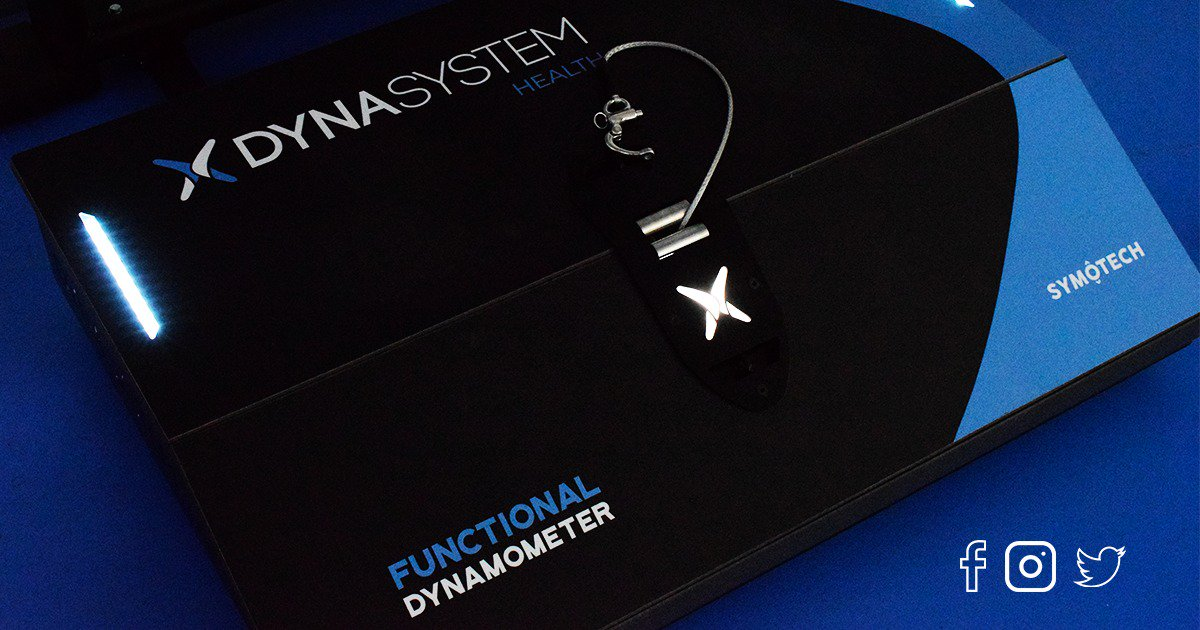
\includegraphics[width=0.7\linewidth]{imagenes/dynasystem-blue-floor.jpeg}
	\caption{Dispositivo DYNAsystem, de la línea \textbf{HEALTH} - \href{https://twitter.com/dynasystem_/status/1001762762111021057}{\textit{Tweet} promocional del producto} [30/05/2018]}
	\label{dynasystem-health}
\end{figure}

Mientras que la apariencia estética será la primera impresión que tendrá del producto un potencial cliente, es necesario que tanto la electrónica interna como el \textit{software embebido} cumplan con su cometido y animen al usuario a seguir utilizando la máquina. Para ello, es de vital importancia que este re-diseño solucione errores de los dispositivos antiguos que comentamos en el apartado anterior, como lo son la \textbf{inestabilidad} (producida quizás por reinicios y/o bloqueos inesperados), la \textbf{latencia} (entendiéndose ésta como retardo en el arranque o la usabilidad) y la \textbf{falta de medios para depuración de errores} (como la ausencia de una consola de administración, o la posibilidad de actualizar remotamente las máquinas vía software). Veamos de forma más directa la descripción del problema, desde un punto de vista funcional y del producto (sin entrar en demasiados detalles técnicos o estructurales), en contraposición con las máquinas antiguas (previamente mencionadas):\\

El dispositivo antecedente a éste se demoraba demasiado en el arranque, inicializando interfaces de red y cargando en memoria la aplicación. Sin embargo, para un caso de éxito, la máquina ha de estar lista para empezar a trabajar con ella lo antes posible desde que se accione su interruptor. Cuanto menos tiempo espere el usuario para configurar su ejercicio, mejor impresión tendrá del producto. Por tanto, es de vital importancia que además de disponer de una infraestructura rápida y ligera, el usuario no tenga que pasar por una pantalla de inicio de sesión como habría de hacerlo en un ordenador convencional.\\

Lógicamente, será necesario que la infraestructura ejecute la aplicación antes mencionada, en torno a la que gira el sistema. Por lo que ésta sufre algún problema o cierre inesperado, el sistema habrá de restaurar su estado (reiniciando automáticamente si la ocasión lo requiere), ya que si el programa no está corriendo, no tendrá sentido que el dispositivo esté en funcionamiento.\\

Durante el tiempo de encendido, el usuario no querrá que su innovador dispositivo le muestre en pantalla una ventana negra de comandos con texto en blanco, por ejemplo, mostrando mensajes del kernel de Linux en carga. Preferiblemente, le gustará ver algún tipo de imagen estática o animada durante el proceso, que desaparezca con dicha aplicación ya preparada.\\

El sistema deberá permitir la conexión a Internet, de forma tanto inalámbrica como cableada, de forma transparente e intuitiva para el usuario. En un futuro se espera tener aplicaciones móviles capaces de tratar los datos emitidos por la máquina, por lo que esta necesidad de conectividad es imperativa.\\

Se espera que se puedan guardar datos brutos generados por la aplicación en un dispositivo de almacenamiento externo (como por ejemplo un \textit{pendrive} o un disco duro convencional).\\

Una de las carencias que sufría el dispositivo implementado por la compañía antigua era la falta de medios de depuración de fallos de software surgidos a lo largo del tiempo. Por tanto, se requiere disponer de un sistema de actualizaciones integrado con el dispositivo que permita solucionarlos de forma remota, ahorrando grandes costes en movilización de servicio técnico.\\

Este protocolo de actualización podrá hacerse mediante red cableada o WiFi (dadas las especificaciones de conectividad de la máquina), y deberá ser lo suficientemente inteligente para saber cuándo una actualización ha sido instalada con éxito; asegurándose de que todo ha ido según lo esperado y retornando a la versión anterior si la nueva impidiese el uso o dejase al dispositivo incomunicado. Por otro lado, dicho sistema de actualizaciones deberá pedir confirmación al usuario antes de aplicar las nuevas instalaciones, de forma que no lo interrumpan en sus ejercicios.\\

El proceso de actualización debe ser fácilmente implementable y llevado a cabo de forma sencilla por una pequeña parte del equipo de desarrollo, que registren los cambios de versiones y desplieguen las actualizaciones desde sus puestos de trabajo.\\

Aunque se espera que el dispositivo tenga diversas formas de administración y/o recuperación, por \textbf{seguridad} es necesario que la entrada de teclado no sea una de ellas; ya que cualquier usuario curioso podría utilizarlo para cerrar la aplicación y manipular el sistema operativo con resultados inesperados.\\

\newpage
	
	% Análisis de requisitos. Estimación de las funcionalidades mínimas y extras (rendimiento, seguridad, disponibilidad, estética). Casos de uso, actores.
	\chapter{Análisis de requisitos}

Una vez tenemos clara la descripción genérica del problema, pasemos a enfocar el problema desde un punto de vista más técnico y agrupemos los requisitos de forma previa a su desarrollo:

\section{Requisitos funcionales}

Para empezar, recopilemos las funcionalidades que deben ser implementadas en el sistema para un correcto desempeño de la aplicación previamente mencionada, dadas las características tan explícitas de ésta:

\begin{itemize}
	\item \textbf{Inicio de sesión automático:} tras cargar el sistema operativo, en lugar de mostrar una terminal o pantalla de inicio de sesión, se deberá acceder al sistema de forma automática con permisos suficientes para ejecutar y cerrar aplicaciones, montar y desmontar interfaces de disco, etc.
	\item \textbf{Ejecución de la aplicación embebida:} el sistema ha de tener el ejecutable del programa instalado en un directorio accesible, con permisos de ejecución para el usuario por omisión.
	\item \textbf{Soporte para conectividad:} la infraestructura a desarrollar debe tener instaladas las dependencias necesarias para proveer al código de la aplicación de binarios útiles para administrar las interfaces de red y sus estados, además de listar las redes disponibles y poder establecer una conexión con éstas.
	\item \textbf{Soporte de almacenamiento externo:} el sistema debe detectar en todo momento que se ha insertado un dispositivo externo, haciendo lo necesario para su montaje y su puesta a punto para el uso de la aplicación. Para esto, será imprescindible que acepte la mayoría de los formatos convencionales actualmente (\textit{NTFS, FAT, exFAT} y \textit{EXTx} entre otros).
\end{itemize}

Vistos dichos requisitos, examinemos los requerimientos de la infraestructura externos a la aplicación, como lo es el \textbf{servicio de actualizaciones}:

\begin{itemize}
	\item El paradigma de despliegue de versiones debe ser fácil de acoplar al sistema y transparente con la aplicación, de forma que ésta sea consciente de la existencia de nuevas versiones y pueda pedir confirmación al usuario. Además, deberán estar centralizadas en un servidor (ya sea local a la empresa o contratado de forma externa); de forma que en lugar de enviarse la actualización individualmente a cada máquina, sean las propias máquinas las que mediante la comunicación con el servidor detecten las potencialmente nuevas versiones.
	\item Para poder realizar actualizaciones atómicas de todo el sistema, será necesario un particionado múltiple. Es decir, el mismo sistema operativo deberá tener dos particiones con sistema de ficheros. Así, mientras una está en ejecución la nueva versión podrá ser instalada en la otra.
	\item Este intercambio de información podrá producirse mediante red cableada o inalámbrica, sin que ello importe al resultado de la operación o dificulte este proceso.
	\item En cada nueva versión del sistema operativo, deberán incluirse las nuevas versiones tanto de la aplicación como del software de la \textbf{electrónica interna} (que se manejaría íntegramente por la aplicación embebida y no ya por la distro en cuestión).
\end{itemize}

Vistas las necesidades del sistema de actualización, veamos ahora un diagrama de estados con el proceso:

\begin{figure}[H]
	\centering
	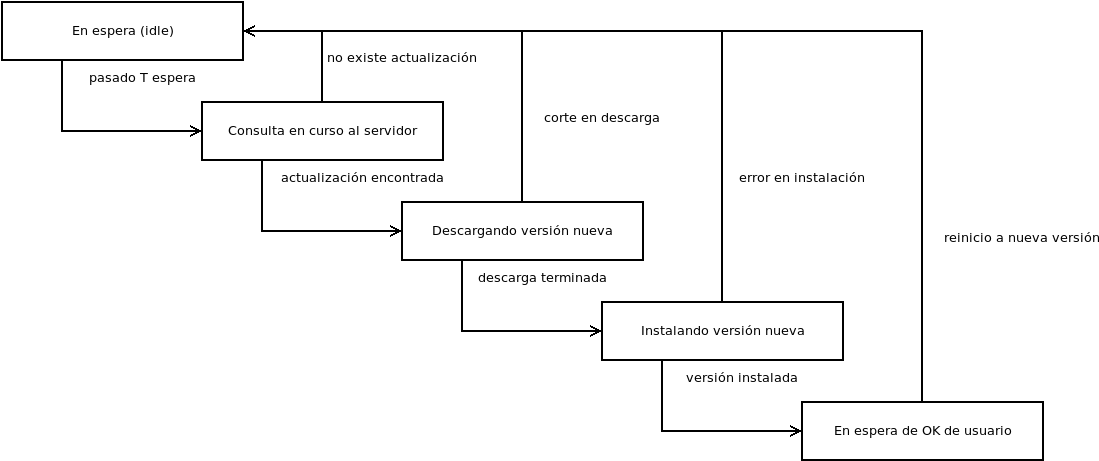
\includegraphics[width=\linewidth]{imagenes/statechart-actualizacion.png}
	\caption{Diagrama de estados del proceso de actualización}
	\label{statechart-actualizacion}
\end{figure}

Una vez definido a petición un período de comprobación de versiones, el cliente se mantendrá a la espera hasta que dicho período se dispare; entonces realizará mediante HTTPS una consulta al servidor, quien le responderá si existe una versión nueva o no.\\

Si no la hay, el cliente vuelve a \textit{``dormirse''}. De lo contrario, comienza la descarga en segundo plano del nuevo software; el cual es instalado en la partición inactiva.\\

Una vez que el usuario da su aprobación mediante la interfaz de la aplicación, o bien cuando decide reiniciar/apagar voluntariamente; la partición marcada como ``activa'' deja de ser la primera. Esto ocasiona que el próximo arranque de la máquina se realice cargando el software más nuevo.\\

Si se produce algún error que impide lanzar la \textit{nueva distro}, o por cualquier motivo no se consigue conectar con el servidor para notificar la actualización realizada, se considera errónea o fallida, volviendo a marcarse la partición antigua como activa y reiniciando al sistema de ficheros antiguo.

\section{Requisitos no funcionales}

Ahora bien, pasemos a ver por otro lado los requerimientos relacionados con las especificaciones de rendimiento, estabilidad, disponibilidad y aspectos estéticos.

\begin{itemize}
	\item En cuanto al \textbf{rendimiento} del sistema, todas las prestaciones de la infraestructura deben centrarse en las acciones del usuario, respondiendo rápido a la interacción táctil, procesando los cálculos internos (de medidas, actualización de gráficas) de manera fluida y eficiente, con los requerimientos de procesamiento gráfico que ello conlleve.
	\item Además, otra parte del rendimiento será el \textit{tiempo de encendido}. Cuanto más ligero sea el sistema operativo y menos (idealmente cero) procesos innecesarios contenga, menor será dicha magnitud. Adicionalmente, la aplicación deberá ser de los primeros servicios en lanzarse, de forma previa al resto de procesos, que lo harán en segundo plano.
	\item Desde el punto de vista de \textbf{la seguridad}, es necesario blindar al sistema intrínseco de cualquier manipulación externa, por lo que el sistema operativo debe ser consciente de si se está ejecutando o no la aplicación en un servicio dedicado, tomando medidas de recuperación cuando no esté haciéndolo (como la re-ejecución del proceso o el reinicio de la máquina). Además, deberá establecerse un proceso que detecte en segundo plano si se ha detectado un teclado, ya que no es de utilidad para la aplicación y cualquier manipulación puede poner en peligro la estabilidad del sistema.
	\item Otro aspecto de la seguridad tiene que ver con las actualizaciones. El motor que las aplique debe controlar de forma exhaustiva cuándo son aplicados correctamente los despliegues, retornando a la versión anterior si no fuese capaz de informar al servidor del éxito en la operación.
	\item Para terminar con los aspectos de protección y recuperación, deberá incluirse en el dispositivo un servidor de administración (del tipo \textit{Secure SHell}) que permita al equipo de desarrollo depurar los posibles errores, así como hacer evaluaciones de rendimiento externas.
	\item Por otro lado, en el apartado \textbf{estético} y pensando en la \textit{computación ubica moderna}, es de imperativa necesidad que el sistema no muestre al usuario los mensajes de la carga que se esté produciendo, ni un modo \textit{línea de comandos} de ningún tipo, de forma que la interfaz sea \textbf{lo más natural posible}. Para ello, deberá modificarse el \textit{bootloader} del computador elegido para que silencie estos mensajes de la salida estándar; además de incluir por otro lado el sistema un servicio que imprima una imagen a pantalla completa, que será reemplazada por la aplicación.
\end{itemize}

Una vez vistos los requerimientos y funcionalidades necesarias del proyecto, pasemos ahora a enumerar y describir los actores involucrados en la vida de dicho producto.

\section{Actores}

Según \textit{Bruce Powel Douglass}, un actor no es más que un objeto (no ya siempre usuarios humanos) fuera del ámbito del sistema bajo estudio, pero que tiene una interacción directa con él \cite{real-time-uml-use-cases}. Por tanto, deberemos ser conscientes de todos los elementos involucrados en el desempeño del proyecto:

\subsubsection{Usuario normal (cliente)}

Es aquel que adquiere la máquina DYNAsystem (o la utiliza en algún gimnasio o centro). Su actuación con respecto a la máquina desde el punto de vista del sistema operativo será sencilla, ya que él simplemente llegará al dispositivo, lo encenderá y visualizará una imagen de carga hasta que aparezca la aplicación embebida, con la que podrá trabajar. Sin embargo, a lo largo de este uso utilizará indirectamente funcionalidades provistas por el sistema operativo, como la reproducción de sonidos indicativos, el guardado de datos a través de USB o la conexión WiFi. Todos estos servicios deberán ser satisfechos por el sistema.

\subsubsection{Programador(es) de la aplicación embebida}

Aunque no participan directamente en esta parte del proyecto (\textit{Meta-DYNAsystem}), para modularizar tareas y que la distribución GNU/Linux siga un desarrollo independiente será necesario el proceso de creación de la aplicación embebida por otro lado, llevado a cabo por el número de personas que la compañía estime necesarias.\\

Estos serán los encargados de abstraerse del sistema Linux y utilizar los módulos provistos por este (de gestión de interfaces de red y de discos, principalmente).

\subsubsection{Administrador(es) del sistema operativo}

Será aquel encargado de analizar, programar y compilar las nuevas versiones del sistema operativo, empaquetando las versiones de la aplicación embebida y el resto del software que se necesite incluir. Para el caso que nos ocupa, dicho puesto lo conformo yo.

\subsubsection{Servidor de actualizaciones}
	
Será el ordenador donde se centralizará todo el servicio de actualizaciones. En este deberán alojarse las imágenes compiladas y será con el que se comuniquen las máquinas (a modo de cliente) para consultar la existencia de nuevas versiones de software.\\

Dependiendo de la implementación del sistema, podrá estar situado en la oficina de la empresa o subcontratado a alguna otra compañía dedicada a la oferta de este tipo de servicios.
	
\newpage

	
	% Alternativas para cada problema y soluciones tomadas al respecto
	\chapter{Decisiones y soluciones}

Una vez están claros los requisitos y se les ha realizado un análisis para su posterior implementación, podemos empezar a comentar las decisiones tomadas y las soluciones implementadas.\\

Pero antes, cabe decir que el principal motivo que me animó a adentrarme en este proyecto fue mi experiencia con muchas distribuciones basadas en \textit{GNU/Linux} adquirida a lo largo de la carrera. Siempre me ha gustado instalarlas en mi ordenador para probarlas, luego desinstalarlas y pasar a probar otras nuevas. Pasar por eso me ha obligado a lidiar con gestores de arranque, administradores de paquetes, configuraciones de sistemas de ficheros y entornos de escritorio, entre otras cosas.\\

Gracias a esto, he podido ver con soltura y abstracción las diferentes piezas de este puzzle llamado \textit{``Meta-DYNAsystem''}, aplicando mis conocimientos previos para desarrollar un sistema lo más robusto posible.\\

Ya venimos hablando largo y tendido sobre dispositivos embebidos, pero es ahora cuando hablaremos de las alternativas elegidas para infraestructura física y virtual, las herramientas de desarrollo de la distribución, y por último del gestor de actualizaciones.

\section{Infraestructura física elegida}

Como anticipábamos en el estado del arte, existen diferentes posibilidades en un proyecto a la hora de desarrollar una infraestructura física que abastezca a un sistema informático:\\

-- Por ejemplo, podríamos optar por montar un ordenador de sobremesa de formato convencional e instalar ahí la infraestructura virtual; dotándola de unas mayores capacidades computacionales, a expensas del precio.\\

-- O por otro lado, encontramos la opción de utilizar un computador \textit{SBC} de los ya mencionados; lo que ajustaría mucho el precio de coste disminuyendo también la potencia máxima del sistema.\\

Para empezar, como comentamos en la descripción del problema, la empresa tenía como premisa reducir los precios de coste del producto original, que llevaba instalado un ordenador convencional en formato \textbf{\textit{Mini-ITX}}.

\begin{quotation}
	\textit{Mini-ITX} es un formato de placa base para ordenadores compactos. Fue desarrollado de forma propietaria por la compañía \textit{VIA Technologies}, desencadenó un gran uso de este formato y posteriormente sus especificaciones pasaron a ser libres \cite{via-mini-itx}.
\end{quotation}

Por una parte, el computador integrado en la máquina antigua disponía de una buena escalabilidad, dado que poseía unas buenas prestaciones. Sin embargo, dichas prestaciones \textbf{no eran necesarias}. Para un sistema dedicado con una sola aplicación embebida, podía utilizarse un ordenador más ajustado tanto en rendimiento como en precio.\\

Por tanto, se pensó en utilizar un computador de placa reducida. Al principio del desarrollo, la empresa propuso utilizar la \textit{Raspberry Pi} descrita previamente (en su versión \textit{3 Model B}, la más avanzada del momento en ese entonces \cite{raspberry-pi-3-model-b}), dado que los dos ingenieros electrónicos que trabajan allí ya la habían utilizado para algunos proyectos y disponían de algunas unidades allí en la oficina. Sin embargo, en todo momento tuve voz y voto en la decisión para plantear alguna otra alternativa.\\

Finalmente, decidimos seguir adelante con ella por diversas razones:

\subsubsection{Relación calidad/precio}

Este suele ser un factor de éxito por el que las \textit{SBC's} han ganado popularidad a lo largo de los años, dado que ofrecen unas prestaciones más que adecuadas para proyectos dedicados ajustando mucho el precio de coste. Las especificaciones son comedidas pero suficientes para un sistema de archivos ligero y aplicaciones sin demasiados requisitos gráficos.\\

Podemos encontrar este tipo de placas por un precio de \textbf{30-40€}, con configuraciones de cuatro núcleos y 1-2 GiB de \textit{RAM}. Suelen disponer de arquitectura \textit{ARM} en el procesador e incluyen \textit{GPU} (unidad de procesamiento de gráficos) cuya memoria es tomada de la \textit{RAM}.\\

Pese a tener estas especificaciones limitadas, provee de todas las conexiones necesarias para el proyecto (puertos \textit{USB}, salida \textit{HDMI}, conexión inalámbrica \textit{Wifi}+\textit{Bluetooth} ya integradas y hasta el puerto de conexión \textit{LAN}). Esto hace que suponga una forma más que interesante de ahorrar costes de manufactura.\\

\subsubsection{Popularidad y comunidad de usuarios}

Aunque a igualdad de precio podríamos haber considerado algunas placas diferentes con las mismas especificaciones, lo que terminó de decantar la balanza por la \textit{Raspberry} fue principalmente la popularidad que posee, así como la amplia comunidad de gente que utiliza estos dispositivos. Esto parece sentenciar que ni el fabricante va a irse a pique, ni se van a encontrar errores en el desarrollo que no haya sufrido ya algún internauta. Es decir, se facilita mucho la búsqueda de ayuda ante posibles errores.\\

Por otro lado, de esta popularidad deriva el grado de soporte para algunos marcos de trabajo. Por ejemplo, \textit{Yocto Project} tiene un alto número de librerías disponibles para desarrollar sistemas embebidos para la \textit{Raspberry}. Y por otro lado, dada esta popularidad el equipo de desarrollo de la herramienta de actualizaciones \textit{Mender} reconoce a esta placa como su dispositivo de referencia \cite{mender-raspberry-pi} (hablaremos de esto más adelante).

\begin{figure}[H]
	\centering
	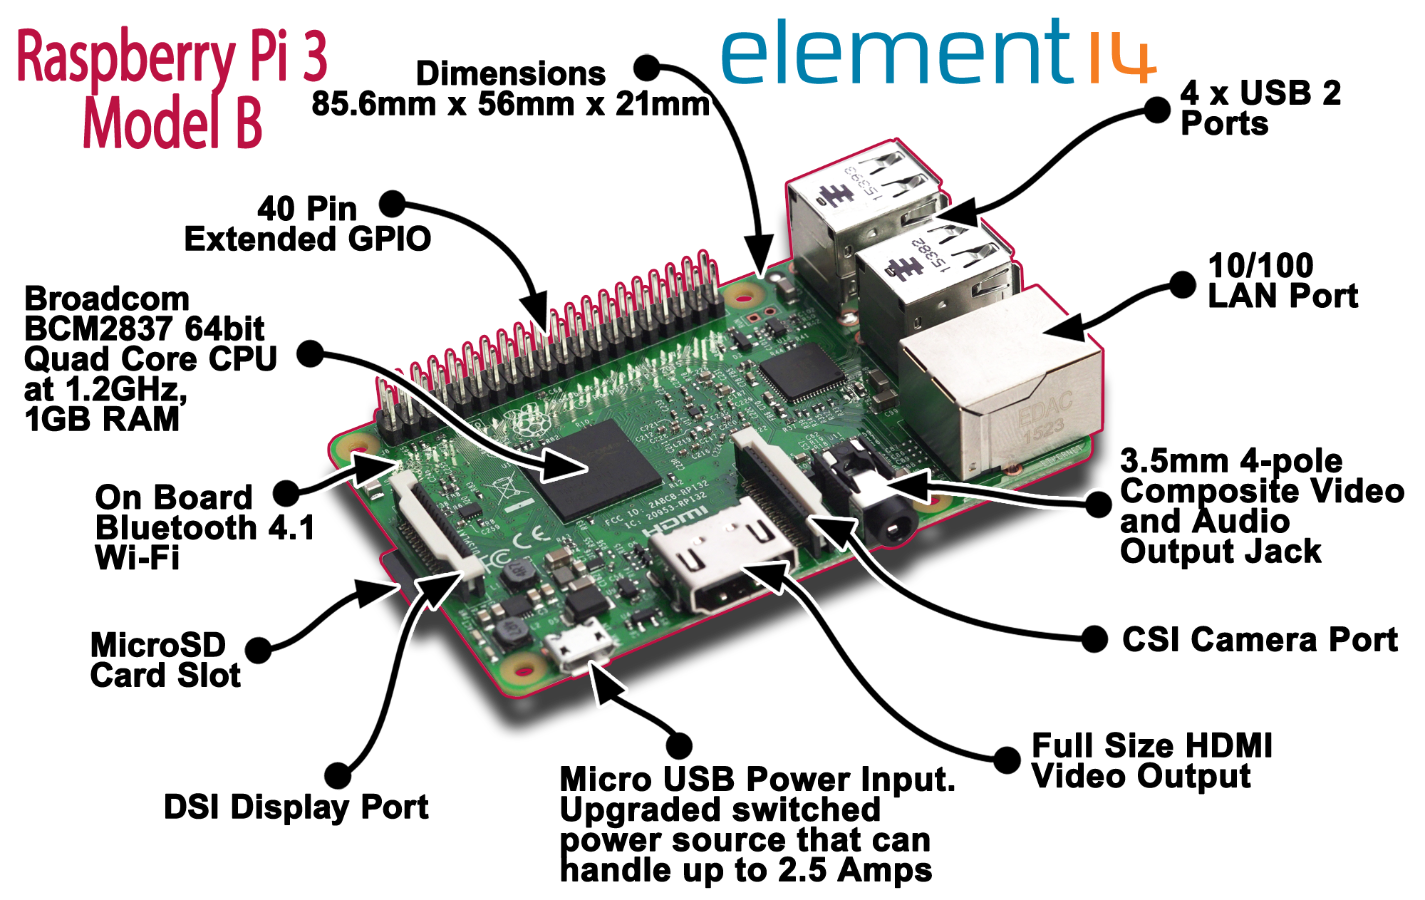
\includegraphics[width=0.9\linewidth]{imagenes/Pi3+Breakout+Feb+29+2016.png}
	\caption{Especificaciones técnicas y conexiones físicas de la \textit{Raspberry Pi 3 modelo B} - \textit{Element 14} \cite{raspberry-pi-3-model-b-specs}}
	\label{rpi3-b-specs}
\end{figure}

\section{Desarrollo del sistema operativo}

Una vez que hemos hablado sobre placas reducidas y microcomputadores, definamos los paquetes de soporte necesarios (\textbf{\textit{BSP, Board Support Packages}}), ya que nos cruzaremos con este término cada vez que queramos desarrollar un sistema operativo basado en una placa específica; y mejor aún, nos permitirá portar un sistema prácticamente idéntico de una arquitectura a otra.\\

Según \textit{Tammy Noergaard} y \textit{Jean Labrosse} \cite{embedded-software-know-it-all-bsp}, se trata de un componente opcional integrado por el proveedor en el sistema operativo, y cuyo propósito principal es proveer de una capa de abstracción entre el sistema operativo y los controladores de dispositivo genéricos.\\

Un \textit{BSP} provee de llamadas al sistema a las capas superiores (las de software) para abstraerlas de los modos del procesador, las tablas de interrupciones y el control de registros.\\

Estos paquetes de soporte nos facilitarán enormemente el desarrollo de un sistema operativo para una placa específica como la \textit{Raspberry Pi}. En el caso de que una empresa quisiera desarrollar todos los aspectos de un sistema empotrado, incluyendo el apartado hardware, los ingenieros electrónicos harían bien en facilitar un \textit{BSP} a los desarrolladores de aplicaciones embebidas que trabajen en el proyecto; dada la facilidad y el ahorro de tiempo que supondrían.\\

\subsection{Elección de la infraestructura software}

En este punto, dejé de tener influencia por parte de la empresa, ya que era el único con conocimientos profundos de \textit{Linux} y era el responsable de valorar las alternativas. No eran demasiadas, ya que las únicas interesantes que encontré fueron \textit{el Proyecto Yocto} (\textit{derivado de Open Embedded}), del que ya venimos hablando; y \textit{Buildroot}.\\

La premisa de ambas herramientas es la de construir un sistema \textit{Linux} completamente personalizado, incluyendo \textit{bootloader} (esto es, la parte de la placa que carga el sistema operativo), \textit{toolchain} (herramientas para el desarrollo de programas sobre la placa) y \textit{kernel} (núcleo \textit{Linux} del sistema operativo). Además comparten la característica de compilar todo íntegramente desde el código fuente público de cada uno de los módulos, utilizando (si es necesario) \textbf{compilación cruzada}. Esto permite compilar programas y módulos en una arquitectura diferente a la del dispositivo final (por ejemplo, el desarrollo de una aplicación embebida podría realizarse en un ordenador \textit{x86\_64} para ejecutarse en una \textit{Raspberry Pi} con arquitectura \textit{ARM}).\\

Veamos una comparación de las dos alternativas de código abierto más grandes para este fin, comentando ventajas e inconvenientes de cada una. Nos apoyaremos en el documento que me ayudó a tomar la decisión, perteneciente a un evento producido en 2016 en el que \textit{Alexandre Belloni} y \textit{Thomas Petazzoni} mostraban las características, potestades y debilidades de cada proyecto \cite{yocto-vs-buildroot-event}:

\begin{figure}[H]
	\centering
	
\includegraphics[width=0.6\linewidth]{imagenes/buildroot_rpi_yocto_logos.jpg}
	\caption{Logos de \textit{Buildroot},\textit{ Raspberry Pi} y \textit{the Yocto Project}} - \cite{imagen-buildroot-rpi-yocto}
	\label{rpi-buildroot-vs-yocto}
\end{figure}

\subsection{Buildroot}

\begin{itemize}
	\item Se enfoca principalmente a la \textbf{simplicidad}, por lo que aunque es sencillo de usar y tiene una curva de aprendizaje no muy grande, no es demasiado extensible.
	\item Se basa en herramientas muy tradicionales como lo son  \textbf{\textit{Kconfig}} (lenguaje de programación para configuración del kernel \cite{kconfig}) y \textbf{\textit{make}} (conocidísima herramienta de compilación por lotes de proyectos \cite{make-tool}).
	\item Muestra una forma muy fácil de configurar el sistema deseado, pues basta con ejecutar \texttt{make menuconfig} para tener una interfaz en modo terminal con la que marcar/desmarcar opciones de paquetes que deberán ser instalados. Esta configuración completa se guarda al completo en un archivo \textit{defconfig}. Finalmente, con lanzar \texttt{make} ya da comienzo la compilación del sistema final.
	\item Si se quiere generar el mismo sistema para arquitecturas diferentes, como por ejemplo una versión de producción para la \textit{Raspberry Pi} y otra de pruebas para virtualizar con \textit{QEMU}, es necesario disponer de dos carpetas de compilación separadas.
	\item Concentra todo el catálogo de paquetes en un solo repositorio oficial, lo que permite una mayor supervisión del código incluido por parte de los expertos pero limita la extensibilidad del proyecto.
\end{itemize}

\subsection{Yocto Project}

\begin{itemize}
	\item Deriva del proyecto \textit{Open Embedded}, que a priori permitía elaborar distribuciones de \textit{Linux} propias solamente para la arquitectura \textit{QEMU} (orientada a virtualización). Sin embargo, una vez conformado el proyecto \textit{Yocto}, da soporte a la mayoría de máquinas.
	\item En cuanto a lenguajes, se basa en \textit{Bitbake} y \textit{Python}. Requiere una curva de aprendizaje mayor y la configuración, que se realiza cómodamente con un editor de texto, es algo más compleja. Sin embargo, permite una mayor libertad al usuario para desarrollar módulos independientes de su interés.
	\item Provee de las dependencias del núcleo pero permite extender funcionalidades, máquinas y código a través de \textbf{\textit{layers}} (entendido en español como \textit{``capas''}). La lista de \textit{layers} puesta a disposición del proyecto se encuentra en \cite{yocto-layers-list}.
	\item Permite crear \textit{layers} independientes para las modificaciones aisladas de cada usuario (de hecho, esta es la forma idónea y más transparente de trabajar con customización de sistemas en Yocto, como aconsejan en el manual \cite{yocto-manual-own-distro}).
	\item Es un proyecto independiente dirigido por la comunidad, pero agrupa a muchos colaboradores de empresas y fabricantes como \textit{Samsung}, \textit{Atmel}, \textit{Raspberry Pi}, \textit{Freescale}, \textit{Asus} y un largo etcétera, que ponen a disposición de los usuarios paquetes \textit{BSPs} de sus placas.
\end{itemize}

Vistas las diferencias, podemos constatar que \textit{Yocto Project} se trata de una alternativa más férrea y profesional, que cuenta con una comunidad numerosa compuesta de gente influyente y activa en el sector. Por si esto fuera poco, tras haber probado ambas alternativas durante un tiempo, es muy notable la flexibilidad que comporta, mientras que su ``rival'' limita mucho a la hora de dar rienda suelta a la creatividad (o mejor dicho, las necesidades) del usuario. Por tanto, el proyecto habrá sido basado en esta alternativa.

\section{Gestor de actualizaciones}

Otra parte importante del proyecto reside en \textbf{las actualizaciones}. Para ser vendido a nivel internacional, \textit{DYNAsystem} necesita disponer de una herramienta de mejora de su software así como de depuración de posibles errores. Además, dichas actualizaciones han de verificar ciertos requisitos de seguridad, asegurando que una instalación fallida no dejaría incomunicada a la máquina o al usuario sin poder trabajar con ella cuando lo quisiese. Por esto, buscaremos especialmente un sistema de actualizaciones con \textbf{soporte para \textit{rollback}}, herramienta que detecta cuando una actualización ha sido realizada correctamente y cuando no, volviendo a la versión anterior para que el dispositivo siga en funcionamiento.\\

Una vez decidida la implementación de un sistema embebido basado en \textit{Yocto} sobre la \textit{Raspberry Pi}, ``tan solo'' es necesario encontrar un gestor de actualizaciones que soporte ambas tecnologías. En la referencia \cite{yocto-system-update} tenemos una lista de las plataformas disponibles en los \textit{layers} antes mencionados. Veamos un resumen de cada una de las alternativas:

\begin{itemize}
	\item \textbf{\textit{swupd}}: distribuye el sistema operativo en (al menos) una sola partición, seleccionando los ficheros que deben ser actualizados. Su código está alojado en el layer \textbf{\textit{meta-swupd}} \cite{meta-swupd} y, según dicha \textit{wiki} del proyecto, resulta ser un sistema bastante fiable y seguro para actualizaciones frecuentes. Sin embargo, no dispone de un sistema por defecto de recuperación frente a errores, lo que le resta peso como alternativa.
	\item \textbf{\textit{sbabic's swupdate}}: también es flexible en cuanto a particionamiento y sus módulos están alojados en \textbf{\textit{meta-swupdate}} \cite{meta-swupdate}. Exige imágenes cifradas y transmitidas mediante \textit{HTTPS}, lo que le transfiere seguridad. Lamentablemente, también necesita de trabajo extra para instalar un sistema de \textit{roll-back}.
	\item \textbf{\textit{Mender}}: se basa en un esquema de cuatro particiones (arranque, sistema de ficheros \#1, sistema de ficheros \#2 y partición de datos persistente); siendo \#1 y \#2 dos sistemas de ficheros inicialmente iguales pero que se irán alternando con la sucesión de actualizaciones. Es decir, cuando una de ellas esté activa y se detecte una actualización, ésta será instalada en la partición en desuso, que se marcará como ``activa'' para el siguiente arranque del dispositivo. También funciona sobre \textit{HTTPS} y permite cifrado de imágenes. Afortunadamente, \textbf{posee soporte para \textit{roll-back}}, por lo que si al iniciar desde la segunda partición no consigue dar parte al servidor de que se ha actualizado, considera fallida la actualización y se vuelve a activar la partición previa. El layer dedicado es \textbf{meta-mender} \cite{meta-mender}, su código es estable y está bajo desarrollo activo.
	\item \textbf{\textit{OSTree}}: al igual que \textit{Mender}, se trata de otra alternativa adecuada para el proyecto; ya que aún siendo flexible en cuanto a particionamiento, contiene soporte de recuperación en cuanto a actualizaciones fallidas, sea por caídas de conexión o de corriente eléctrica. Tiene una base de usuarios significativa y un ciclo de desarrollo rápido en su capa \textbf{\textit{meta-updater}} \cite{meta-updater}.
	\item \textbf{\textit{RAUC}}: también flexible en cuanto a bloques de dispositivo, exige que las imágenes comprimidas viajen firmadas con el protocolo \textit{X.509}. Tiene disponible la función de \textit{rollback} siempre y cuando el \textit{bootloader} integrado la soporte. Sus módulos están disponibles en \textbf{meta-rauc} \cite{meta-rauc}.
\end{itemize}

Una vez vistas las alternativas, constatamos que las más interesantes son las tres últimas, dado que permiten recuperación del sistema en caso de error o actualización fallida. Sin embargo, la diferencia vendrá dada por el modo de centralización de las diferentes versiones, pudiendo ser repositorios de código aislado o servidores propios debidamente administrados.\\

Con respecto a esto, la empresa desarrolladora de \textit{Mender} (\textit{Northern Tech} \cite{northern-tech}) ofrece una alternativa de pago más que interesante: \textbf{\textit{Hosted Mender}}, que consiste en la puesta a punto y el mantenimiento de un servidor donde alojar las actualizaciones, y con el que comunican cada uno de los dispositivos clientes. Partiendo de esto, el desarrollador solo tiene que preocuparse de integrar el sistema operativo con la comunicación al servidor, así como de ir subiendo las imágenes cifradas a dicho servidor y finalmente eligiendo en el portal web los dispositivos a los que se quiere desplegar la imagen actualizada. Esta alternativa permite a la empresa ahorrar el tiempo de un ingeniero dedicado a la administración del servidor, y por lo tanto el coste que ello supone.\\

Por otro lado, en \textbf{\textit{meta-mender}} \cite{meta-mender} disponemos de la lista de paquetes y utilidades necesarias para dicha integración, mientras que en la documentación \cite{docs-mender} encontramos los pasos requeridos para ello; que utilicé para realizar las pruebas con este software. Dado que \textit{Hosted Mender} permitía una fase beta gratuita de pruebas, dediqué tiempo a experimentar con este software, intercambiando correos con los responsables cuando me surgía alguna duda al respecto, quienes me respondieron y ayudaron de buena gana. Finalmente, decidí optar por esta alternativa, ya que cumplía todas las expectativas y, tras comentarlo con mi empresa, decidimos que era la mejor opción en cuanto a resultados, tiempo y dinero.

\newpage

	
	% Distribución propia de GNU/Linux basada en Yocto Project. Puesta a punto del proyecto, enumeración de las tareas para satisfacer los requisitos.
	\chapter{Implementación del sistema operativo}

Una vez que sabemos las decisiones tomadas y las tecnologías utilizadas, pasemos a estudiar cada una de las soluciones implementadas en confrontación con los requisitos estudiados.\\

Empezaremos por la puesta a punto del sistema de compilación y continuaremos con la configuración necesaria para el funcionamiento esperado del sistema operativo embebido. Dado el volumen del proyecto Yocto, describiremos solo parcialmente sus factores de configuración y el proceso de trabajo con él.

\section{Introducción y puesta a punto}

Como venimos mencionando a lo largo de la memoria, el proyecto Yocto se basa en la herramienta \textit{Open Embedded} y en el lenguaje de configuración \textit{Bitbake}, que permite ajustar desde parámetros del kernel hasta elegir paquetes que no se quiere sean instalados. Además, cabe destacar que se pueden compilar imágenes con Yocto de diversas formas, ya sea utilizando contenedores aislados (a modo de máquinas virtuales) o nuestro propio sistema Linux \textit{anfitrión}, como vemos en la documentación de inicio \cite{yocto-project-quick-start-build-system}. Por mi parte, siempre he preferido hacerlo en el propio sistema, dado que así se destinan a la compilación el 100\% de los recursos asignados disponibles y el tiempo de espera es menor.\\

Para el caso que nos ocupa, la versión utilizada del proyecto Yocto ha sido la \textbf{2.4} (de nombre \textit{Rocko}), dado que se trataba de la versión estable más avanzada en el momento del desarrollo.\\

La guía relativa a la puesta a punto la encontramos en el manual \textit{Quick Start} de la web \cite{yocto-project-quick-start} ya mencionado, y consiste principalmente en instalar las dependencias necesarias para nuestra distribución y clonar mediante \texttt{git} el núcleo del proyecto, llamado \textit{Poky}, con el comando siguiente (la opción \texttt{-b} elige la rama deseada):

\begin{center}
\texttt{git clone git://git.yoctoproject.org/poky -b rocko}
\end{center}

\subsection{Manipulación y compilación de prueba}

Una vez tenemos el núcleo, lo siguiente es empezar a configurar el resultado que queremos obtener. Si ejecutamos el comando \texttt{source oe-init-build-env}, se nos generará un directorio destino \textit{build} con una configuración de ejemplo para una máquina \textit{Qemu} de 32 bits.\\ 

La premisa de este tipo de sistemas de desarrollo es incluir lo mínimo para funcionar, y que sea el desarrollador quien elija las dependencias a incluir. Por tanto, aunque dicho archivo de configuración es grande, se trata de mucho código de ejemplo y comentarios de ayuda al recién llegado.\\

Aquí podemos elegir entre cambiar el dispositivo de destino y los paquetes a instalar, o seguir adelante con una imagen mínima de prueba de la siguiente forma:

\begin{center}
\texttt{bitbake core-image-minimal}
\end{center}

El nombre \texttt{core-image-minimal} hace referencia a la imagen de menor tamaño por defecto, por lo que para hacer pruebas es suficiente. \\

\subsection{Variables de configuración del sistema}

La sintaxis de configuración es sencilla, y sigue la forma: 

\begin{center}
	\texttt{PARÁMETRO\_CONFIGURACIÓN = "valor deseado"}
\end{center}

En el directorio \textit{build} antes creado, podremos ir incorporando configuración al archivo \textit{conf/local.conf} con dicha sintaxis de la herramienta \textit{Bitbake} para instalar/borrar paquetes del dispositivo.\\

La sintaxis de código para añadir dependencias sería la siguiente (hemos de añadir esta línea al archivo \textit{conf/local.conf} mencionado):

\begin{center}
\texttt{IMAGE\_INSTALL\_append = `` <paquete1> <paquete2> ...''}
\end{center}

Si quisiéramos eliminar alguno de los paquetes incluidos por alguna librería necesaria, es tan fácil como sustituir \texttt{append} por \texttt{remove}.\\

Por otro lado, si profundizamos en los archivos de configuración descargados de cualquiera de los layers, encontramos en alguna ocasión configuración de la forma:

\begin{center}
\texttt{VARIABLE ?= "valor"}
\end{center}

Cuando un símbolo de interrogación acompaña a esta variable, significa que es un \textbf{valor por defecto}, fácilmente anulable por una asignación sin dicho símbolo en cualquier parte.\\

Por ejemplo, en la configuración por defecto, el dispositivo por destino se muestra tal que así:

\begin{center}
\texttt{MACHINE ?= "qemux86"}
\end{center}

En nuestro caso, borraremos la interrogación y escribiremos ``raspberrypi3'' entre comillas, dado que es nuestro dispositivo elegido (podemos consultar el listado completo en \href{http://layers.openembedded.org/layerindex/branch/master/machines/?q=&browse=1}{OpenEmbedded Layer Index}, junto con los layers necesarios para cada máquina).\\

\subsection{Layers y librerías}

Por otro lado, la forma de reutilizar librerías y capas ya existentes es sencilla. Podemos encontrar la lista completa de capas y paquetes pertenecientes a éstas en la referencia \cite{yocto-layers-list}. Para empezar basta con descargarlas (también mediante \texttt{git}) en el directorio raíz del sistema de compilación. Acto seguido, añadimos una línea en el fichero \texttt{./build/conf/bblayers.conf} con la ruta a la librería descargada. [\textit{bblayers} toma su nombre por \textit{Bitbake Layers}.] Hecho esto, el comando \texttt{bitbake} detectará todos los paquetes y dependencias que tenemos importados en el sistema, viéndose esto reflejado en cada compilación.\\

En la web antes mencionada, \url{https://layers.openembedded.org}, dentro de la sección \textbf{\textit{Recipes}} podemos buscar paquetes que nos interesen, dando con la(s) capa(s) que los incluyen. Por ejemplo, si quisiéramos utilizar \textit{PSplash}, una herramienta para imprimir imágenes de carga embebidas, obtendríamos lo siguiente:

\begin{figure}[H]
	\centering
	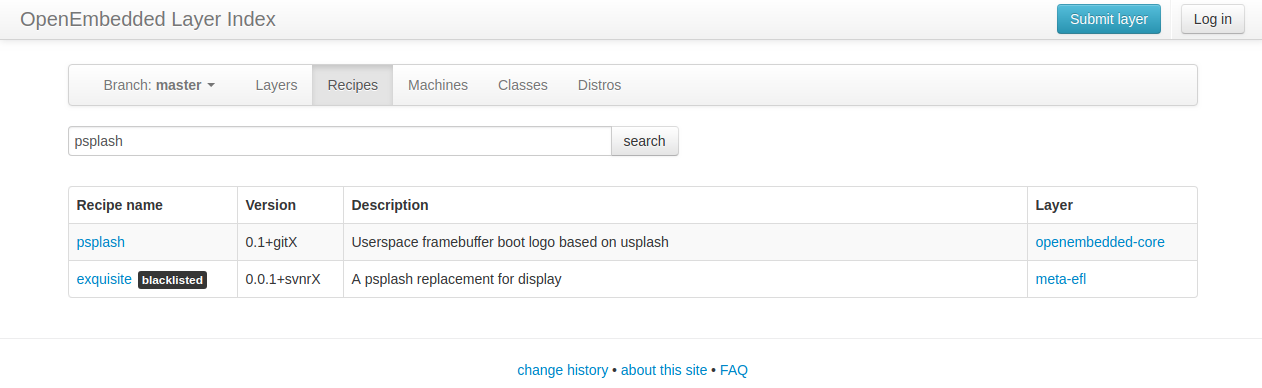
\includegraphics[width=\linewidth]{imagenes/yocto-recipe-search-example.png}
	\caption{Ejemplo de búsqueda en las recetas de OpenEmbedded [13/06/2018]}
	\label{yocto-recipe-search-example}
\end{figure}

Como vemos, los resultados vienen compuestos del nombre de los paquetes, las versiones (para filtrar cuando existen varias del mismo), una descripción inteligible y el layer donde encontrarlo. Si hacemos click en el nombre del layer, veremos una descripción de dicha capa y la dirección del repositorio donde se aloja (y que habremos de clonar).\\

\subsubsection{Layer propio}

Como aconsejan en la propia documentación de Yocto, una vez que queremos pasar de hacer pruebas a confeccionar nuestro producto, lo idóneo es \textbf{crear un \textit{layer} propio} en el que alojar la configuración de forma aislada. Por ejemplo, en nuestro caso la capa usada recibe el nombre de \texttt{meta-dynasystem} y da nombre a este proyecto.\\

Los pasos para crear un layer, descritos en la propia \textit{Wiki} de Yocto \cite{wiki-yocto-own-layer}, son sencillos. El proceso consiste básicamente en generar un par de carpetas y un archivo de configuración común al layer (llamado \textit{layer.conf}), describiendo las rutas internas a la capa y la prioridad de sus paquetes con respecto a los de otras.\\

Por otro lado, debemos saber que dentro de cada layer existirán distintos directorios 

\begin{itemize}
	\item \textbf{Configuración propia del layer \textit{(/conf)}}: el archivo necesario se aloja en la ruta antes mencionada \texttt{./conf/layer.conf}.
	\item \textbf{Ficheros de clases \textit{(/classes)}}: las clases representan comportamientos específicos que pueden heredar las imágenes de sistema. Tienen extensión \texttt{.bbclass}.
	\item \textbf{Recetas de paquetes de todo tipo \textit{(/recipes-X)}}: siendo ``X'' variable y reflejando el tipo de las recetas que se usan. Por ejemplo, los paquetes importantes o las imágenes suelen ser incluidas en una carpeta llamada \textbf{\textit{recipes-core}}; o las recetas relacionadas con Mender se agrupan en la carpeta \textbf{\textit{recipes-mender}}.
\end{itemize}

Dentro de estas carpetas de recetas encontraremos un directorio por cada paquete de la categoría. Comentemos esto en el siguiente apartado.\\

\subsection{Paquetes, configuración y parches}

Como hemos dicho anteriormente, encontramos una carpeta para cada paquete existente, con el mismo nombre del paquete. De forma interna a esta, podremos distinguir varios subdirectorios y archivos:

\begin{itemize}
	\item \textbf{Archivos a incluir en el sistema \textit{(/files)}}: aquí se alojan ficheros de todo tipo que se quiere figuren en el sistema final asociados al paquete (scrips, documentos, etc.).
	\item \textbf{Parches por aplicar al paquete \textit{(/patches)}}: comentaremos su función de forma más extensa en esta sección más adelante.
	\item \textbf{Configuración adicional para el paquete \textit{(paquete\_\%.bbappend)}}: <paquete> se refiere al nombre, y ``\%'' simboliza el número de versión. En este archivo se hace referencia a los ficheros del directorio \textit{/files} y los parches de \textit{/patches} que se quieren tomar en consideración.
\end{itemize}

Para terminar con la introducción a Yocto, cabe destacar la importancia de \textbf{los parches} previamente mencionados (o \textit{patches} en inglés). Estos permitirán de una forma escalable y, sobre todo automatizada, modificar el comportamiento de las aplicaciones y programas libres ya presentes en los repositorios.\\

Para entender el funcionamiento de los parches, veamos antes los estados por los que pasa un paquete por compilar:

\begin{enumerate}
	\item Se descarga el código fuente de la aplicación. El repositorio desde el que se descarga vendrá especificado por el fichero \textbf{\textit{``receta.bb''}} propio del paquete. Por ejemplo, la receta del paquete PSplash \cite{yocto-recipe-psplash}. La variable que almacena el enlace se llama \texttt{SRC\_URI}.
	\item Los layers pueden aplicar configuración y parches al código descargado de otros layers, guardando estas modificaciones en archivos \textbf{\textit{``receta.bbappend''}}. Después del primer paso, para cada paquete se buscan todos los ficheros \textit{.bbappend} que le correspondan, y se aplican las modificaciones oportunas.
	\item Una vez aplicados todos los parches, se compila el código completo y se incluye para ser instalado en la imagen de destino.
\end{enumerate}

Esto representado en UML en forma de diagrama de estados sería tal que así:

\begin{figure}[H]
	\centering
	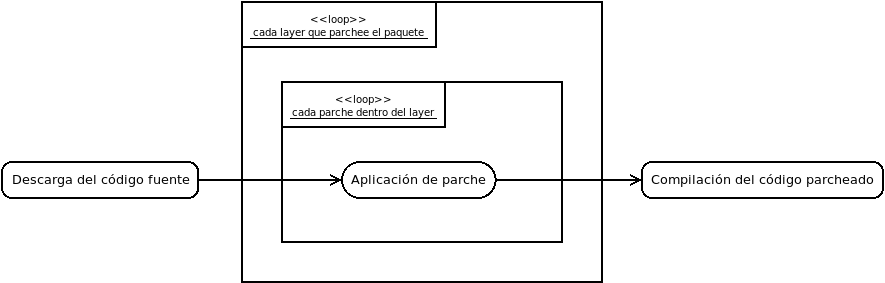
\includegraphics[width=\linewidth]{imagenes/statechart-parche.png}
	\caption{Diagrama de estados por los que pasa una dependencia en Open Embedded}
	\label{statechart-parche}
\end{figure}

\noindent\makebox[\linewidth]{\rule{\textwidth}{0.4pt}}\\

\subsubsection{Proceso de parcheo de paquetes}

Por otro lado, un recién llegado al proyecto podría pensar que la forma de redefinir comportamientos en paquetes ya existentes consiste en:

\begin{enumerate}
	\item Hacer en otro repositorio un \textit{fork} del programa en cuestión.
	\item Realizar las modificaciones pertinentes de forma aislada.
	\item Crear una receta en Yocto que obtenga el paquete desde el nuevo repositorio, con prioridad mayor al original.
\end{enumerate}

Yo mismo probé a hacerlo durante un tiempo, pero a pesar de que esto realmente puede llegar a ``funcionar'', es desacertado, pues además de ser lento y arduo no aporta escalabilidad ni automatización de ningún tipo.\\

La forma escalable de trabajar viene dada por \textbf{la herramienta \textit{devtool}}, que genera una copia local del código fuente del programa listo para que realicemos las modificaciones pertinentes. Además, nos permitirá realizar compilaciones utilizando esta versión temporal, para verificar el funcionamiento de los cambios añadidos. Encontramos la guía de estos pasos en la referencia \cite{wiki-yocto-patches}.\\

Ejecutamos \texttt{devtool nombre\_del\_paquete} y la herramienta descargará el código fuente, le serán aplicados todos los parches de las capas existentes por parte de \textit{bitbake}, y será generada una carpeta \texttt{./build/tmp/sources/nombre\_del\_paquete} con este código final.\\

Sobre el código de este directorio será sobre el que hagamos las modificaciones. Para probar estos cambios, bastará con compilar el paquete de forma aislada (\texttt{bitbake nombre\_del\_paquete}) y ejecutarlo.\\

\subsubsection{Inclusión de parches en layer propio}

Cuando terminemos con las pruebas y queramos guardar los cambios realizados, deberemos generar un archivo en forma de parche interpretable de forma automática por Bitbake, y que quede de forma persistente en nuestro propio layer.\\

Bitbake detectará automáticamente la existencia de estos parches y los aplicará al código fuente del programa antes de compilarlo e instalarlo en la imagen de destino. Para desarrollar sistemas con Yocto, es una de las mecánicas más usadas, ya que generalmente existen paquetes para casi cualquier necesidad que tengamos, pero siempre están abiertos a modificaciones más especiales.\\

El comando de generación de parches es simple y conocido, dado que no es específico de Bitbake sino de GNU/Linux. Para el caso de un parche a un paquete genérico, el comando tendría la siguiente estructura:\\

\textit{\textbf{git diff ./build/tmp/sources/<paquete>/<fichero\_modificado> \\./<layer\_propio>/recipes-<X>/patches/<paquete>.patch}}\\

\noindent\makebox[\linewidth]{\rule{\textwidth}{0.4pt}}\\

Una vez que tenemos el parche generado e importado en nuestro layer, necesitaremos hacer ver a la receta original del paquete parcheado la existencia de dichas modificaciones. Para ello crearemos una receta del tipo \textit{.bbappend} como las ya antes mencionadas, con el siguiente contenido:

\begin{lstlisting}
FILESEXTRAPATHS_prepend := "${THISDIR}/patches:"
\end{lstlisting}

Esto provocará que Bitbake automáticamente tenga en cuenta estos cambios y los incorpore sobre el código original del paquete.\\

Una vez hayamos hecho esto, podremos centrarnos en los paquetes utilizados y/o desarrollados para satisfacer las necesidades del producto.

\section{Desarrollo de los paquetes necesarios}



\subsection{Sistema mínimo}


\texttt{POR EXPLICAR:\\
	- autologin\\
	- arranque silencioso (no terminal)\\
	- [seguridad] no entrada teclado\\
	- [seguridad] no ejecución sin aplicación (watcher)\\
	- [actualizaciones] salvar redes wifi\\
	- [app] ejecución de la aplicación embebida\\
	- [app] librerías de qt\\
	- [actualizaciones] actualizacion interna de la electronica\\
	- conectividad inalámbrica (wifi \& bluetooth)\\
	- soporte de audio\\
	- pantalla completa durante carga\\
	- ficheros. soporte para usb's (formatos ntfs, fat, exfat)\\
	- [actualizaciones] actualización a través de servidor\\
	- [actualizaciones] confirmación por parte del usuario}\\

\section{Integración con el gestor de actualizaciones}

Por explicar integración con Mender, paquetes necesarios, etc.

\newpage
	
	% Caso de éxito y uso real
	\chapter{Casos de éxito y uso real del producto}

El módulo \textit{Meta-DYNAsystem} se pensó para ser desarrollado en un plazo de tres meses, uno de aprendizaje y dos de producción real de código e implementación del proyecto.\\

Sin embargo, el tiempo de desarrollo de la aplicación embebida, desarrollada por otro lado por otra parte del equipo, llevó más tiempo. Para entonces, la distribución propia basada en \textit{GNU/Linux} ya estaba terminada.\\

El producto pudo ser \textbf{lanzado al mercado y comercializado a nivel global}, siendo adquirido por clientes que llevaban tiempo siguiendo de cerca el proyecto a la espera del lanzamiento. Esto quiere decir que tanto el dispositivo al completo como su sistema operativo dedicado intrínseco se están utilizando a día de hoy en un ambiente de producción de uso diario.\\

Pasemos a hablar sobre los \textbf{primeros compradores}. Se trata del \textbf{equipo de investigación de \textit{Ciencias del Deporte} de la \textit{Universidad Católica de la Santísima Concepción}} \textit{(Chile)}.\\

Estos usuarios ya disponen de su dispositivo enviado e instalado en sus centros de investigación, utilizando el sistema a diario para extraer datos en tiempo real del entrenamiento de sus deportistas. Veamos un par de imágenes:

\begin{figure}[H]
	\centering
	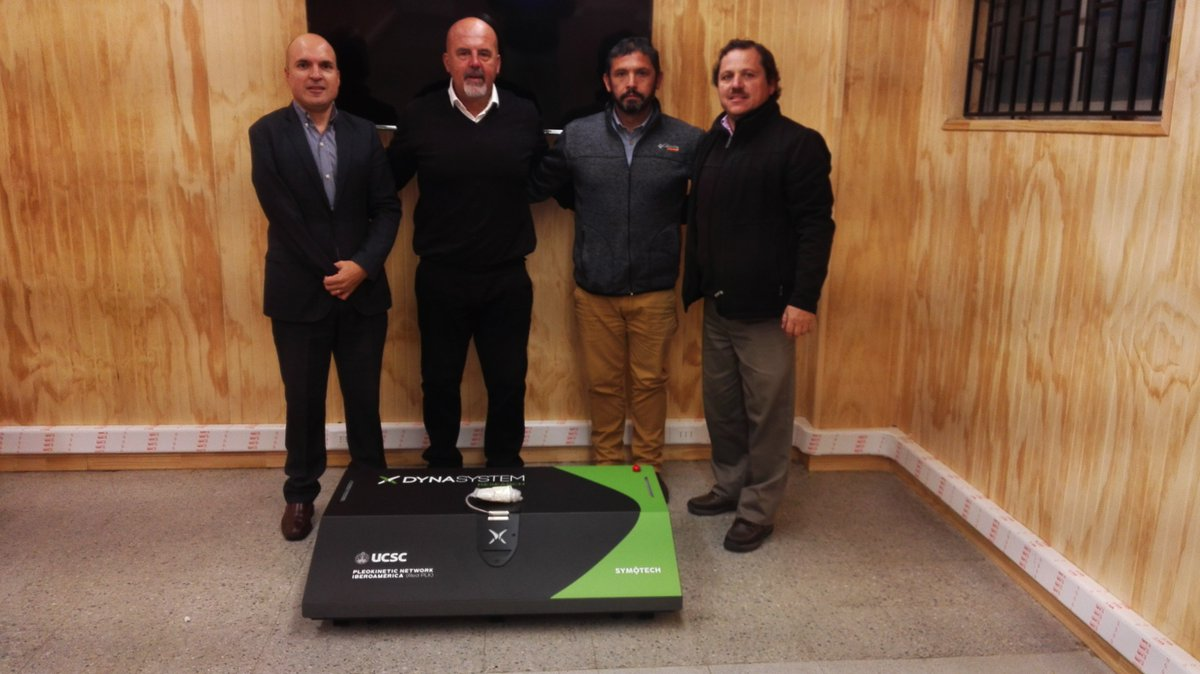
\includegraphics[width=0.9\linewidth]{imagenes/dynasystem-ucsc.jpg}
	\caption{Máquina \textit{DYNAsystem} adquirida por el equipo de investigación de Ciencias del Deporte de la \textit{UCSC (Chile)} - \textit{Twitter} oficial del producto \cite{dynasystem-ucsc}}
	\label{dynasystem-ucsc}
\end{figure}

\begin{figure}[H]
	\centering
	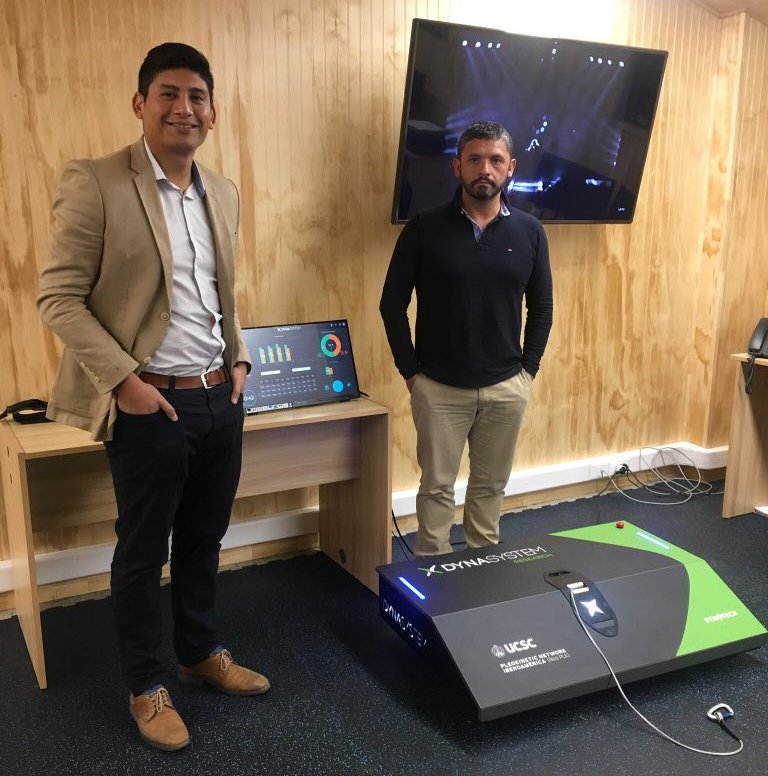
\includegraphics[width=0.7\linewidth]{imagenes/dynasystem-ucsc-2.jpg}
	\caption{Máquina \textit{DYNAsystem} adquirida por el equipo de investigación de Ciencias del Deporte de la \textit{UCSC (Chile)} - \textit{Twitter} oficial del producto \cite{dynasystem-ucsc-2}}
	\label{dynasystem-ucsc-2}
\end{figure}

Por otro lado, durante las primeras semanas de uso del dispositivo en Chile, en el equipo de desarrollo de \textit{Symotech} se siguieron implementando mejoras y avances en las capacidades del dispositivo, además de solucionar algunos errores conocidos de no demasiada importancia.\\

Gracias al sistema de actualizaciones integrado con la distribución interna al dispositivo, \textbf{se pudieron desplegar dos actualizaciones exitosas de forma remota}; actualizando tanto el software intrínseco a la electrónica como la aplicación embebida con que interacciona el usuario.\\

Veamos una captura de pantalla de la plataforma web de \textit{Hosted Mender}, servicio ya comentado previamente, donde se aprecia el éxito de la actualización finalizada.\\

En ella se muestra parte del ID del dispositivo, su tipo (basado en \textit{Raspberry Pi 3}), la versión actualmente instalada y las fechas de inicio y finalización del despliegue:

\begin{figure}[H]
	\centering
	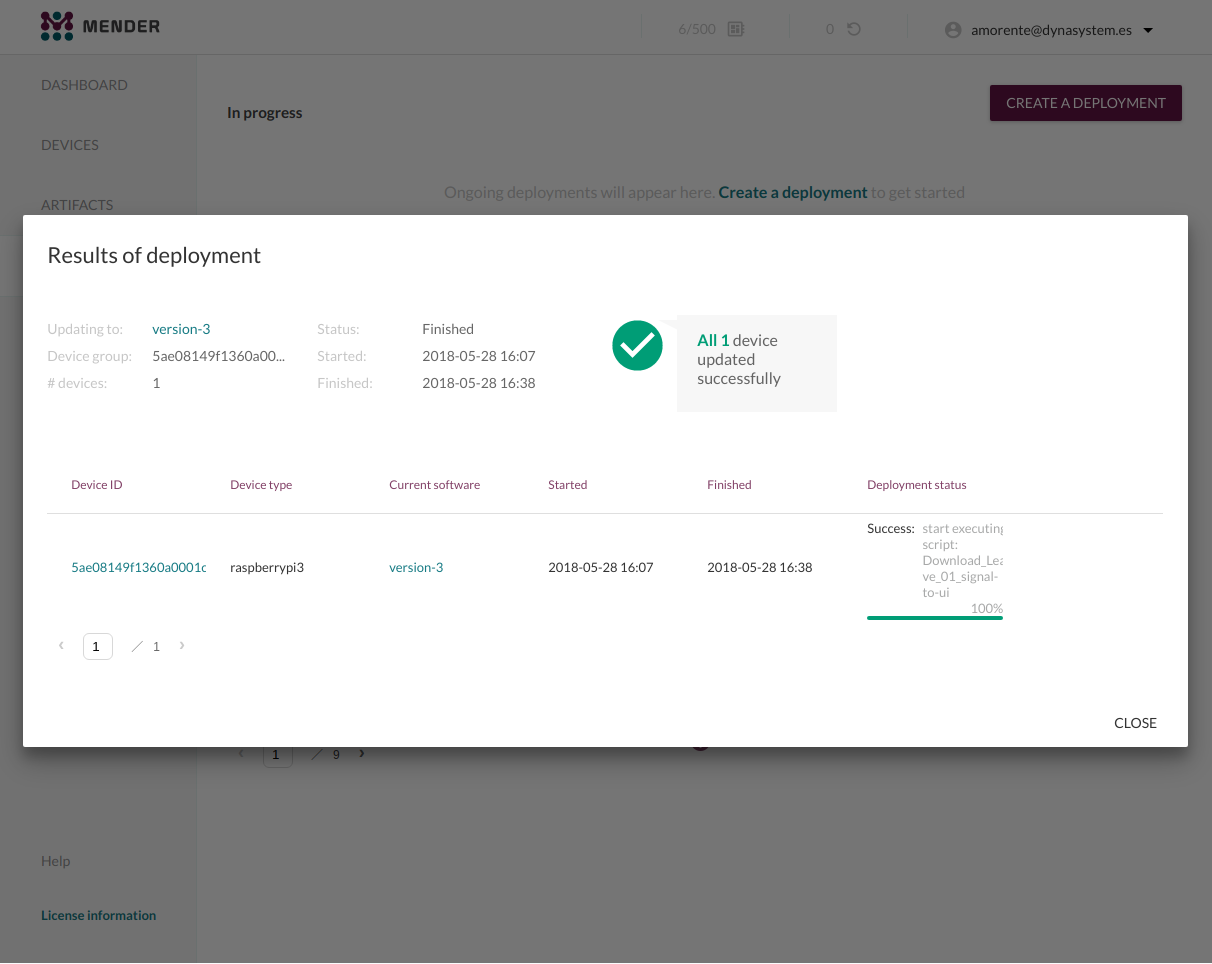
\includegraphics[width=\linewidth]{imagenes/ejemplo-actualizacion-exitosa.png}
	\caption{Muestra de la segunda actualización exitosa a la máquina instalada en la \textit{UCSC} de Chile - Adrián Morente Gabaldón \textit{[plataforma web de Hosted Mender]}}
	\label{dynasystem-ucsc-mender}
\end{figure}

\noindent\makebox[\linewidth]{\rule{\textwidth}{0.4pt}}\\

Actualmente, a mediados de junio de 2018, se han producido más ventas e instalaciones del dispositivo a nivel nacional con actualizaciones realizadas, pero no disponemos de medios de carácter multimedia que lo prueben (como imágenes o vídeos).\\

Sin embargo, en la ya mencionada cuenta de \textit{Twitter} oficial del producto se pueden encontrar muchos medios de publicidad y difusión del dispositivo, con gente ajena al proyecto (fisioterapeutas y deportistas de todo tipo) probándolo a diario y dando su visto bueno: \href{https:www.twitter.com/dynasystem\_}{enlace a \textit{Twitter}} \cite{twitter-dynasystem}.

\newpage
	
	% Presupuesto del proyecto completo para propósito general.
	\chapter{Presupuesto del proyecto}

Pasemos ahora a realizar una estimación lo más acertada posible del coste de implantación del proyecto. Independientemente de haber sido pensado para su integración con \textit{DYNAsystem}, el contenido desarrollado podría aprovecharse para su uso en otro tipo de sistemas dedicados, modificando tan solo la imagen de carga y la aplicación embebida (y otras dependencias, si se quiere). Finalmente, haremos la distinción presupuestaria de lo que supone para una empresa (o desarrollador) llevar a cabo el proyecto en cuanto a \textbf{producción}, y por otro lado el que sería un precio justo de venta al público.\\

Empecemos por la parte física con \textbf{el hardware final}, que aunque proporcionalmente apenas supone coste merece una apreciación:

\begin{itemize}
	\item Por un lado tenemos el \textbf{computador de placa reducida}. En este caso se trata de la ya tan mentada \textit{Raspberry Pi} aunque podría adaptarse a otra placa (cambiando algunos drivers específicos). Ya mencionamos que los argumentos por los que principalmente se decidió desarrollar un sistema embebido sobre este tipo de dispositivos fue por \textbf{consumo}, en contraposición a las prestaciones; y \textbf{precio}, dado que esta gama suele oscilar siempre en torno a los \textbf{30-40€} \cite{raspberry-pi-amazon} y cumple nuestras necesidades de rendimiento sin problema.
	\item Por otro lado, necesitaremos una \textbf{tarjeta de memoria} en formato \textit{Micro SD} donde instalar el sistema operativo. Aquí las restricciones no vendrán dadas por el tamaño, dado que la imagen completa ocupa poco más de 400 \textit{MiB}; sino por \textbf{la velocidad}, que repercutirá directamente en la lectura de datos en la carga del sistema. Con una de estas memorias de la clase 10 (mínimo 10 \textit{MB/s}) bastaría sin problema. En cuanto al rango de precios, nos moveremos entre los \textbf{5 y 12€} según el tamaño que elijamos, aunque no sea necesario en su totalidad.
\end{itemize}

A este precio habremos de sumarle siempre un coste, sea del tiempo dedicado a realizar el pedido por Internet mas los gastos de envío; o bien al coste de movilidad del personal hasta un comercio donde adquirir dichos componentes. Pongamos esta cifra en \textbf{10€}, a modo de estimación.\\

Esto concluye con que tendríamos la infraestructura física final por \textbf{cerca de 60€}.\\

\noindent\makebox[\linewidth]{\rule{\textwidth}{0.4pt}}\\

Finalmente, volviendo a hablar del desarrollo del proyecto como parte del sistema embebido \textit{DYNAsystem}, cabe destacar que aún \textbf{no está perfectamente definido el precio de coste de producción de la empresa para estos dispositivos}. Sin embargo, podemos afirmar sin temor a equivocarnos que la implantación del computador de placa reducida con la distribución de \textit{GNU/Linux} instalada supone un porcentaje ínfimo del coste total (quizás entre un 4 y 5\% del precio de producción).

\noindent\makebox[\linewidth]{\rule{\textwidth}{0.4pt}}\\

Por otro lado, aunque no se incluye dentro del final, una parte de hardware necesaria para llevar a cabo el proyecto será el centro de trabajo donde el ingeniero desarrolle el sistema (es decir, el ordenador con el que se realizarán las compilaciones). En cualquiera de los componentes a mentar podría incrementarse el precio si buscamos un resultado por encima de la media, pero en cuanto a gamas estándar y en base al mercado actual, estimemos de forma muy general la cifra necesaria:

\begin{itemize}
	\item Para empezar, el monitor. Sin ser demasiado exquisitos, partiendo de uno de 24 pulgadas con resolución \textit{FullHD} y un resultado más que correcto, el precio partiría de \textbf{130-140€} \cite{monitor-samsung-pccom}, llegando a 300 si se buscase una configuración con doble monitor, o uno solo con mayores resoluciones y tamaños.
	\item Por otro lado, el ordenador en sí. El ingeniero no necesitará realizar cómputos relacionados con gráficos sino que hará un gran desempeño del procesador y de la memoria (tanto volátil como persistente). Para esto, un procesador \textit{Intel} \textit{i5} o \textit{i7} acompañado de 8 \textit{GiB} de memoria \textit{RAM} y 2 \textit{TiB} de disco duro serían más que suficientes. Esta configuración sumaría \textbf{750-800€} al total \cite{ordenador-sobremesa-pccom}.
	\item Para terminar con las herramientas necesarias, un combo de teclado y ratón, que en una gama estándar podría conseguirse por \textbf{20€} (o hasta \textbf{60} si buscamos un resultado más profesional con teclados mecánicos, inalámbricos o retroiluminados) \cite{combo-teclado-logitech-pccom}.
\end{itemize}

Finalmente, la estación de trabajo del desarrollador tendría un coste de entre \textbf{1.000} y \textbf{1.300€} para un caso genérico.\\

Ahora bien, utilizando este hardware dedicará un número de horas de trabajo variable según las especificaciones del proyecto. Para este caso, podría estimarse una temporalidad de \textbf{1 a 2 meses de trabajo, para un contrato de 40 horas semanales}, y en función de su experiencia con \textit{Open Embedded} y \textit{Yocto Project}.\\

Haciendo también una estimación del salario a tiempo completo del ingeniero (pongamos que oscila entre 1.200 y 1.800€), concluiríamos que el precio de coste total de producción sería el siguiente:

\begin{quotation}
	\textbf{Mínimo estimado\textit{}}: (1 mes) x (1.200€ de salario) + (1.000€ de ordenador) + (60€ de placa) = \textbf{2.260€}\\
	
	\textbf{Máximo estimado\textit{}}: (2 mes) x (1.800€ de salario) + (1.300€ de ordenador) + (60€ de placa) = \textbf{4.960€}
\end{quotation}

Como decimos, en esta cifra influyen muchas variables, desde el precio de los componentes hasta el salario del desarrollador, pero podemos fijar el intervalo del \textbf{precio de coste de producción entre 2.000 y 5.000€}. 

\noindent\makebox[\linewidth]{\rule{\textwidth}{0.4pt}}\\

Una vez que se tienen las herramientas de trabajo y una cierta mecanización del desarrollo por parte del ingeniero, podemos hacer números para estimar un Precio de Venta al Público correcto.\\

Con las medidas precedentes ya tomadas, adaptar el desarrollo de un proyecto dado a otro distinto no requeriría rehacer muchas cosas, ya que las bases con \textit{Open Embedded/Yocto Project} son siempre las mismas; por lo que a petición de un cliente, se podría realizar el proyecto solicitado en un tiempo de \textbf{un mes a tiempo completo} (40 horas semanales).\\

Tomemos la hora de trabajo de un ingeniero a un precio de venta de 50€, y hagamos la estimación del Precio de Venta al Público:

\begin{quotation}
	\textbf{P.V.P. estimado}: (40 horas) x (50€ cada hora) = \textbf{2.000€}
\end{quotation}

\textbf{2.000€} sería el precio estimado de venta al público de un proyecto basado en este para cada mes de trabajo dedicado.

\newpage
	
	% Conclusión del proyecto
	\chapter{Conclusión}

fuentes de información válidas y fiables

planificación temporal realista de las actividades

oportunidades para hacer nuevas propuestas

caracterizar situación práctica reconociendo los conocimientos que demanda

diferentes opciones para generar alternativas de solución

profundizar en tareas asignadas cumpliendo los objetivos programados

revisar sistemáticamente el trabajo

aspectos éticos y sociales relacionados con la profesión

\newpage
	
	\newpage
	\bibliography{citas}
	\bibliographystyle{plain}
	
\end{document}
